%%%%%%%%%%%%%%%%%%%%%%%%%%%%%%%%%%%%%%%%%%%%%%%%%%%%
% Instructivo para trabajar este documento en Overleaf
%
% 1. Crear un nuevo proyecto en Overleaf en blanco.
%
% 2. Crear una carpeta llamada "resources":
%    - En la barra lateral izquierda, haz clic en el ícono de carpeta.
%    - Haz clic en el botón "New Folder".
%    - Escribe el nombre: resources
%    - Presiona Enter o el botón "Create"
%
% 3. Subir la imagen "universidad-del-valle.png" a la carpeta "resources":
%    - Haz clic derecho sobre la carpeta "resources" recién creada.
%    - Selecciona "Upload".
%    - Elige el archivo "universidad-del-valle.png" desde tu computadora.
%
% 4. Copiar documento
%    - Elimina todo el contenido del archivo main.tex, copia y pega en él todo el contenido del presente documento
%
% 5. Compilar con el botón "Recompile" o Ctrl + s
%%%%%%%%%%%%%%%%%%%%%%%%%%%%%%%%%%%%%%%%%%%%%%%%%%%%


%%%%%%% PAQUETES Y CONFIGURACIONES %%%%%%% INICIO
\documentclass[11pt,letter]{article}

% Idioma y codificación
\usepackage[utf8]{inputenc}
\usepackage[spanish]{babel}

% Diseño de página
\usepackage[left=2.54cm,right=2.54cm,top=2.54cm,bottom=2.54cm]{geometry}
\usepackage{setspace}
\usepackage{float}

% Tipografía y matemáticas
\usepackage{amsmath}
\usepackage{pifont}

% Colores (debe ir antes de tcolorbox y pgfplots)
\usepackage[table,xcdraw]{xcolor}

% Gráficos y figuras
\usepackage{graphicx}
\usepackage{pgfplots}
\pgfplotsset{compat=1.18}

% Tablas y cajas
\usepackage{booktabs}
\usepackage[most]{tcolorbox}
\usepackage{mdframed}
\usepackage{adjustbox}

% Algoritmos y código
\usepackage[linesnumbered,ruled,vlined]{algorithm2e}
\renewcommand{\listalgorithmcfname}{Lista de Algoritmos}
\renewcommand{\algorithmcfname}{Algoritmo}
\usepackage{listings}


% Referencias y notas
\usepackage{nameref}
\usepackage{natbib}
\usepackage{endnotes}
\usepackage[backend=biber,style=apa]{biblatex}
\addbibresource{bibliografia.bib}

% Hipervínculos (último siempre que sea posible)
\usepackage{hyperref}

%Para dar ancho a tabla
\usepackage{tabularx}

% Centrado de tablas
\usepackage{array}
\newcolumntype{C}[1]{>{\centering\arraybackslash}m{#1}} % Centrado horizontal y vertical

\definecolor{verde}{RGB}{199,233,192}
\definecolor{rosado}{RGB}{255,199,206}
\definecolor{grisazul}{RGB}{218,227,243}
\definecolor{grisclaro}{RGB}{242,242,242}
\usepackage{colortbl}
\usepackage{graphicx}
\usepackage{xcolor}
\usepackage{array}
\usepackage{float}
\usepackage{multirow}

%%%%%%% PAQUETES Y CONFIGURACIONES %%%%%%% FIN


\begin{document}
    \onehalfspacing

%%%%%%% PORTADA %%%%%%% INICIO
    \begin{titlepage}
        \centering
        
\includegraphics[width=0.15\textwidth]{resources/universidad-del-valle.png}\par\vspace{1cm}
        {\scshape\LARGE Universidad del Valle \par}
        {\scshape\Large Facultad de Ingeniería \par}
        {\scshape\Large Escuela de Ingeniería de Sistemas y Computación \par}
        \vspace{2cm}

        {\Large \textbf{Moderando el Conflicto Interno de Opiniones en una Red Social}}\\

        \vspace{2cm}
        {\large \textbf{Anderson Johan Alban Angulo - 202310006}}\\
        {\large \textbf{Andrés Felipe Asprilla Urrutia - 202224101 }}\\
        {\large \textbf{Andrés Mauricio Ortiz Bermúdez - 202110330}}\\
        {\large \textbf{Carlos Mauricio Tovar Parra - 201741699}}\\
        \vspace{2cm}

        \Large\textbf{Profesor}\par
        {\large \textbf{Jesús Alexander Aranda Bueno Ph.D.}}\\
        \vspace{1.4cm}
        \Large\textbf{Curso}\par
        {\large \textbf{Análisis y Diseño de Algoritmos II (750020C)}}\\
        \vspace{1cm}
        {\large {19 de abril de 2025}\par}
    \end{titlepage}
%%%%%%% PORTADA %%%%%%% FIN

%%%%%%% INDICE %%%%%%% INICIO
    \tableofcontents
    \newpage
    \listoftables
    \newpage
    \listoffigures
    \newpage
    \listofalgorithms

%%%%%%% INDICE %%%%%%% FIN
    \newpage

%%%%%%% INTRODUCCIÓN %%%%%%% INICIO


    \section{Introducción}

    En este proyecto se aborda el problema de la moderación del conflicto interno de opiniones en una red social ficticia, denominada ModCI. Este fenómeno se presenta cuando un mismo individuo sostiene opiniones inconsistentes frente a dos afirmaciones relacionadas con un mismo tema, lo que refleja una falta de coherencia interna. Esta incoherencia puede ser indicativa de una comprensión superficial o confusa del tema, y su presencia generalizada en una red social puede afectar la calidad del debate y la estabilidad de las posturas colectivas.
    \par\vspace{0.5cm}
    El objetivo principal del proyecto es diseñar e implementar soluciones algorítmicas que permitan reducir el conflicto interno de la red social, modificando las opiniones de algunos de sus agentes de manera estratégica, teniendo en cuenta el nivel de rigidez de cada uno y un presupuesto limitado de esfuerzo disponible. Para ello, se utilizaron y compararon tres enfoques clásicos del diseño de algoritmos: fuerza bruta, algoritmos voraces y programación dinámica.
    \par\vspace{0.5cm}
    Cada enfoque será aplicado al problema ModCI para identificar qué agentes deben ser priorizados en el proceso de ajuste de opinión, con el fin de maximizar la reducción del conflicto interno total en la red. Además de implementar los algoritmos, se realizará un análisis comparativo considerando la optimalidad de las soluciones y la eficiencia computacional de cada estrategia.
    \par\vspace{0.5cm}
    Este proyecto busca que los estudiantes pongan en práctica las técnicas aprendidas para enfrentar problemas de naturaleza combinatoria, y que sean capaces de evaluar críticamente las ventajas y limitaciones de diferentes enfoques algorítmicos, tanto desde el punto de vista teórico como práctico.
%%%%%%% INTRODUCCIÓN %%%%%%% FIN

    \newpage

%%%%%%% FUNCIONES AUXILIARES %%%%%%% INICIO


    \section{Funciones auxiliares}

    Se implementaron varias funciones auxiliares que permiten calcular de manera modular el esfuerzo de moderación aplicado a una red social y el conflicto interno resultante. Estas funciones son esenciales para evaluar cualquier estrategia de solución (fuerza bruta, voraz o dinámica).

    \[
        \begin{aligned}
            \textbf{CI} &: \text{Conflicto Interno} \\
            \mathcal{RS} &: \text{Red Social} \\
            o_{i,1} &: \text{Primera opinión del grupo } i \\
            o_{i,2} &: \text{Segunda opinión del grupo } i \\
            r_i &: \text{Rigidez del grupo } i \\
            E &: \text{Estrategia de moderación}
        \end{aligned}
    \]


    \subsection*{1. \texttt{calcular\_conflicto}}
    Esta función estima el nivel de conflicto interno de una red social, considerando una posible estrategia de moderación. Si no se proporciona una estrategia, se asume que todos los agentes conservan sus opiniones originales. El cálculo sigue la definición de conflicto interno:

    \[
        CI(\mathcal{RS}) = \frac{\sum_{i=0}^{n-1} \left(n_i^\mathcal{RS} \ast \left(o_{i,1}^\mathcal{RS} - o_{i,2}^\mathcal{RS}\right)^2\right)}{n}
    \]

    donde $e_i$ es la cantidad de agentes moderados del grupo $i$. El conflicto se promedia respecto al número total de grupos

    \begin{itemize}
        \item \textbf{Entrada:} \texttt{red\_social} (lista de tuplas), \texttt{estrategia} (lista opcional).
        \item \textbf{Salida:} Valor del conflicto interno (real).
    \end{itemize}

    \subsection*{2. \texttt{calcular\_esfuerzo}}
    Calcula el esfuerzo total requerido para aplicar una estrategia de moderación sobre los grupos de la red. El esfuerzo se calcula como:

    \[
        Esfuerzo(\mathcal{RS}, E) = \sum_{i=0}^{n-1} \left[ \left| o^{\mathcal{RS}}_{i,1} - o^{\mathcal{RS}}_{i,2} \right| * r^{\mathcal{RS}}_i * e_i \right]
    \]


    \begin{itemize}
        \item \textbf{Entrada:} \texttt{red\_social}, \texttt{estrategia}.
        \item \textbf{Salida:} Esfuerzo total requerido (entero).
    \end{itemize}

    \subsection*{3. \texttt{calcular\_ci\_esfuerzo}}
    \label{sec:calcular_ci_esfuerzo}
    Función compuesta que retorna simultáneamente el conflicto interno y el esfuerzo total asociado a una estrategia. Es usada como función de evaluación principal por los tres enfoques de solución.

    \begin{itemize}
        \item \textbf{Entrada:} \texttt{red\_social}, \texttt{estrategia}.
        \item \textbf{Salida:} Tupla \texttt{(conflicto, esfuerzo)}.
    \end{itemize}

    \subsection*{4. \texttt{extraer\_datos\_red}}
    Facilita la manipulación de la red social al extraer sus atributos en listas separadas.

    \begin{itemize}
        \item \textbf{Entrada:} \texttt{red\_social}.
        \item \textbf{Salida:} Cuádrupla de listas: \texttt{(n, opiniones\_1, opiniones\_2, rigidez)}.
    \end{itemize}

%%%%%%% FUNCIONES AUXILIARES %%%%%%% FIN
    \newpage
%%%%%%% FUERZA BRUTA %%%%%%% INICIO


    \section{Algoritmo Fuerza Bruta}

    \subsection{Descripción}
    El enfoque de fuerza bruta para resolver el problema ModCI consiste en examinar exhaustivamente todas las posibles formas en que puede distribuirse el esfuerzo disponible entre los grupos de agentes de una red social, con el fin de minimizar su conflicto interno. Este enfoque parte de la premisa de considerar cada combinación factible de cambios en las opiniones de los agentes, evaluando en cada caso el nivel de conflicto resultante. De todas las estrategias que respetan el límite de esfuerzo permitido, se elige aquella que produce el menor conflicto interno. Al contemplar el espacio completo de soluciones, este método asegura encontrar la solución óptima. No obstante, su principal desventaja radica en el elevado costo computacional que implica, lo que restringe su uso práctico a redes de tamaño reducido.

    \subsection{Implementación}
    La implementación del algoritmo de fuerza bruta se realizó empleando una representación estructurada de la red social como una lista de tuplas. Cada tupla modela un grupo de agentes e incluye cuatro elementos: la cantidad de individuos en el grupo, sus opiniones frente a dos afirmaciones específicas, y su nivel de rigidez al cambio de opinión.

    El proceso se estructura en dos fases principales:

    \begin{enumerate}
        \item \textbf{Generación Exhaustiva de Estrategias:} Se construye el conjunto completo de combinaciones posibles de moderación sobre los grupos de agentes. Para cada grupo, se consideran todos los valores enteros desde 0 hasta el número total de agentes del grupo, lo cual representa cuántos de sus miembros podrían modificar su opinión. Al combinar estas posibilidades para todos los grupos, se genera el espacio total de estrategias viables.S
        \item \textbf{Evaluación y Selección de la Mejor Estrategia:} Cada combinación es evaluada mediante la función auxiliar \nameref{sec:calcular_ci_esfuerzo}, la cual calcula tanto el conflicto interno como el esfuerzo requerido para esa estrategia. Si el esfuerzo total no supera el máximo permitido $\mathtt{R_{\text{max}}}$ y el conflicto interno es menor al mejor encontrado hasta el momento, se actualiza la mejor solución.
    \end{enumerate}

    El resultado final es una tupla que contiene: el conflicto interno mínimo alcanzado, el esfuerzo total utilizado y la estrategia óptima de asignación de esfuerzos.

    \subsection{Pseudocódigo}
    \begin{algorithm}[H]
        \caption{modciFB: Estrategia óptima por fuerza bruta}
        \KwIn{Una red social $RS$ como lista de tuplas $(n_i, op1_i, op2_i, rigidez_i)$ para cada grupo $i$, y un esfuerzo máximo permitido $R_{max}$}
        \KwOut{Tupla $(CI_{\min}, Esfuerzo_{\text{total}}, Estrategia_{\text{óptima}})$}

        $mejorCI \leftarrow \infty$ \tcp*[r]{Inicializa el conflicto mínimo como infinito}
        $mejorEsfuerzo \leftarrow 0$ \tcp*[r]{Inicializa el esfuerzo asociado}
        $mejorEstrategia \leftarrow []$ \tcp*[r]{Inicializa la mejor estrategia vacía}

        $estrategias \leftarrow [[]]$ \tcp*[r]{Lista inicial con una estrategia vacía}

        \ForEach{grupo $g_i$ en $RS$}{
            $nuevasEstrategias \leftarrow []$ \\
            \ForEach{estrategia en estrategias}{
                \For{$e \leftarrow 0$ \KwTo $n_i$}{
                    $nuevasEstrategias.\text{append}(estrategia + [e])$
                }
            }
            $estrategias \leftarrow nuevasEstrategias$ \tcp*[r]{Actualizar todas las combinaciones}
        }

        \ForEach{estrategia $E$ en estrategias}{
            $(CI, esfuerzo) \leftarrow calcular\_ci\_esfuerzo(RS, E)$ \\
            \If{$esfuerzo \leq R_{max}$ \textbf{and} $CI < mejorCI$}{
                $mejorCI \leftarrow CI$ \\
                $mejorEsfuerzo \leftarrow esfuerzo$ \\
                $mejorEstrategia \leftarrow E$
            }
        }

        \Return $(mejorCI, mejorEsfuerzo, mejorEstrategia)$
    \end{algorithm}


    \definecolor{lightgray}{rgb}{0.9,0.9,0.9}
    \lstset{
        language=Python,
        backgroundcolor=\color{lightgray},
        frame=single,
        rulecolor=\color{black}
    }

    \subsection{Complejidad}

    \subsubsection{Complejidad Temporal}

    El algoritmo de fuerza bruta tiene una complejidad temporal exponencial, debido a que genera y evalúa todas las posibles combinaciones de esfuerzos para los grupos de la red. Si hay $n$ grupos y cada grupo tiene $k_i$ personas, entonces el número total de combinaciones posibles es:

    \[
        O\left(\prod_{i=1}^{n}(k_i + 1)\right)
    \]

    En el peor de los casos, si todos los grupos tienen un tamaño máximo de $k$, la complejidad se puede expresar como:

    \[
        O\left((k + 1)^n\right)
    \]

    Además, para cada combinación se evalúa el conflicto interno y el esfuerzo total, lo que implica un recorrido lineal sobre los $n$ grupos. Por lo tanto, la complejidad final del algoritmo es:

    \[
        O\left(n (k + 1)^n\right)
    \]

    Esto lo convierte en un algoritmo extremadamente costoso computacionalmente, ya que el tiempo de ejecución crece exponencialmente con el número de grupos y el tamaño de cada uno. Aunque garantiza una solución óptima, este enfoque no es adecuado para instancias grandes del problema.

    En términos prácticos, esta complejidad significa que incluso para valores moderados de $n$ y $k$, el número total de combinaciones puede volverse inmanejable. Por ejemplo, si se tienen apenas 10 grupos de tamaño 10, el algoritmo tendría que evaluar $(10 + 1)^{10} = 25937424601$ combinaciones posibles.

    \subsubsection{Complejidad Espacial}

    La complejidad espacial también es considerable. El algoritmo almacena en memoria todas las combinaciones posibles de esfuerzos antes de evaluarlas. Por tanto, en el peor de los casos, el número de combinaciones almacenadas es:

    \[
            {O}\left((k+1)^n\right)
    \]

    donde $n$ es la cantidad de grupos y $k$ el número máximo de agentes por grupo. Esto se debe a que se construye la lista completa de estrategias (vectores de tamaño $n$), en la cual cada componente puede tomar un valor entre $0$ y $k$.

    Este costo espacial es resultado del uso de listas auxiliares que mantienen todas las estrategias posibles en memoria antes de su evaluación, lo que puede saturar rápidamente la memoria en problemas con muchos grupos o agentes.

    \subsection{Corrección}

    El algoritmo de fuerza bruta desarrollado para el problema ModCI garantiza la
    obtención de la solución óptima, ya que evalúa exhaustivamente todas las
    combinaciones posibles de distribución de esfuerzos entre los grupos de la red
    social. Para cada combinación generada, calcula el nivel de conflicto interno
    resultante y verifica que el esfuerzo total no supere el límite máximo permitido.
    Posteriormente, selecciona la estrategia que logra minimizar el conflicto interno
    dentro de las restricciones establecidas.

    Sin embargo, aunque el algoritmo es correcto desde el punto de vista funcional, su
    ejecución implica una búsqueda exhaustiva de soluciones que conlleva una
    complejidad exponencial. A medida que aumenta el número de grupos o el tamaño
    de estos, el número de combinaciones crece de forma drástica, lo cual impacta
    negativamente en el rendimiento. Esto limita su aplicabilidad a redes de pequeño
    tamaño, donde aún es viable computacionalmente.
    Por lo tanto, si bien este enfoque asegura una solución óptima y es útil como
    referencia o para validar la calidad de soluciones aproximadas, no es práctico para
    redes sociales grandes, y por ello es necesario acudir a técnicas más eficientes
    como los algoritmos voraces o la programación dinámica para abordar instancias
    más complejas del problema.

    \subsection{Análisis}

    A continuación se presenta un análisis concreto que permite ilustrar el funcionamiento paso a paso del algoritmo de fuerza bruta
    \par\vspace{1cm}
    \textbf{Datos de entrada:}

    \begin{table}[ht]
        \centering
        \begin{tabular}{cccccc}
            \toprule
            \textbf{Grupo} & \textbf{Agentes} & \textbf{Opinión 1} & \textbf{Opinión 2} & \textbf{Rigidez} \\
            \midrule
            1              & 1                & -4                 & 2                  & 0.1              \\
            2              & 4                & 1                  & -1                 & 0.2              \\
            3              & 3                & 3                  & 0                  & 0.5              \\
            \bottomrule
            $R_{\text{max}} = 5$
        \end{tabular}
        \caption{Datos entrada: análisis fuerza bruta}
    \end{table}


    \subsubsection*{Análisis del proceso}
    El paso a paso para generar la solución en el algoritmo de fuerza bruta es el siguiente:
    \begin{enumerate}
        \item \textbf{Generación de combinaciones posibles}: Se generan todas las combinaciones de esfuerzos posibles para los grupos, respetando el rango desde 0 hasta el número de agentes por grupo.

        En este caso:
        \begin{itemize}
            \item Grupo 1: $0$ a $1$ (2 opciones)
            \item Grupo 2: $0$ a $4$ (5 opciones)
            \item Grupo 3: $0$ a $1$ (2 opciones)
        \end{itemize}

        Total de combinaciones: $2 \times 5 \times 2 = 20$

        \item \textbf{Cálculo del conflicto interno (CI)}: Se calcula el conflicto interno para cada combinación válida, considerando cuántos agentes permanecen sin moderar. Usando la función \nameref{sec:calcular_ci_esfuerzo}.
        \item \textbf{Cálculo del esfuerzo total por combinación}: Se calcula el esfuerzo total requerido usando la misma función auxiliar.

        \item \textbf{Filtrado por esfuerzo máximo permitido ($R_{\text{max}}$)}: Se descartan combinaciones cuyo esfuerzo supere el valor de $R_{\text{max}} = 5$.

        \item \textbf{Selección de la mejor estrategia}: De las combinaciones válidas, se selecciona la que genere el menor conflicto interno.
    \end{enumerate}

    \textbf{Combinaciones posibles (20 en total):}

    \begin{center}
        \renewcommand{\arraystretch}{1.2}
        \begin{table}[H]
            \centering
            \renewcommand{\arraystretch}{1.2}
            \begin{tabular}{cccc}
                \toprule
                \textbf{Combinación (G1 - G2 - G3)}  & \textbf{Esfuerzo Total} & \textbf{Conflicto Interno} & \textbf{Válida} \\
                \midrule
                0 - 0 - 0                            & 0                       & 45.3333                    & \ding{51}       \\
                0 - 0 - 1                            & 3                       & 33.3333                    & \ding{51}       \\
                0 - 1 - 0                            & 2                       & 40.0000                    & \ding{51}       \\
                0 - 1 - 1                            & 5                       & 28.0000                    & \ding{51}       \\
                0 - 2 - 0                            & 4                       & 34.6667                    & \ding{51}       \\
                0 - 2 - 0                            & 7                       & 22.6667                    & \ding{55}       \\
                0 - 3 - 0                            & 5                       & 29.3333                    & \ding{51}       \\
                0 - 3 - 1                            & 8                       & 17.3333                    & \ding{55}       \\
                0 - 4 - 0                            & 7                       & 24.0000                    & \ding{55}       \\
                0 - 4 - 1                            & 10                      & 12.0000                    & \ding{55}       \\
                1 - 0 - 0                            & 1                       & 33.3333                    & \ding{51}       \\
                \rowcolor{gray!10}\textbf{1 - 0 - 1} & \textbf{4}              & \textbf{21.3333}           & \ding{72}       \\
                1 - 1 - 0                            & 3                       & 28.0000                    & \ding{51}       \\
                1 - 1 - 1                            & 6                       & 16.0000                    & \ding{55}       \\
                1 - 2 - 0                            & 5                       & 22.6667                    & \ding{51}       \\
                1 - 2 - 1                            & 8                       & 10.6667                    & \ding{55}       \\
                1 - 3 - 0                            & 6                       & 17.3333                    & \ding{55}       \\
                1 - 3 - 1                            & 9                       & 5.3333                     & \ding{55}       \\
                1 - 4 - 0                            & 8                       & 12.0000                    & \ding{55}       \\
                1 - 4 - 1                            & 11                      & 0.0000                     & \ding{55}       \\
                \bottomrule
            \end{tabular}
            \caption{Combinaciones posibles fuerza bruta}
        \end{table}
    \end{center}
    \newpage
    \subsection*{Resultados Finales del Algoritmo}

    \begin{table}[H]
        \centering
        \begin{tabular}{|l|c|}
            \hline
            \rowcolor[HTML]{EFEFEF}
            \textbf{Métrica}    & \textbf{Valor}  \\
            \hline
            Estrategia óptima   & {[}1, 0, 1{]}   \\
            \hline
            Conflicto interno   & 21.3333         \\
            \hline
            Esfuerzo total      & 4               \\
            \hline
            Tiempo de ejecución & 0.0039 segundos \\
            \hline
        \end{tabular}
        \caption{Resultados obtenidos: análisis fuerza bruta.}
    \end{table}

    Este ejemplo ilustra cómo el algoritmo de fuerza bruta explora exhaustivamente todas las posibles combinaciones de esfuerzos para encontrar la que minimice el conflicto interno. Aunque este enfoque garantiza encontrar la solución óptima, tiene una complejidad exponencial, ya que el número de combinaciones crece rápidamente con cada grupo o incremento de agentes.

    En esta prueba con solo 3 grupos y 20 combinaciones, el tiempo de ejecución fue casi instantáneo, lo que demuestra que para problemas pequeños es muy efectivo. Sin embargo, en problemas reales con muchos grupos o agentes, este enfoque se vuelve inviable por el alto costo computacional, siendo recomendable en esos casos el uso de algoritmos voraces o programación dinámica.

    \subsection{Impacto en el Rendimiento}
    \label{sec:limitaciones_fuerza_bruta}

    A pesar de su simplicidad, el enfoque de fuerza bruta presenta importantes limitaciones prácticas. Una de las más críticas es el impacto que tiene sobre el rendimiento a medida que crece el tamaño de la red social o el número de agentes por grupo.

    Supongamos que la red social está compuesta por \( n \) grupos, y que cada grupo \( i \) tiene \( a_i \) agentes. Como las estrategias posibles para cada grupo van desde moderar 0 hasta \( a_i \) agentes, entonces el número de combinaciones de estrategias posibles es:

    \[
        \prod_{i=1}^{n} (a_i + 1)
    \]

    Este crecimiento es exponencial en el número de grupos, y además está influenciado por el tamaño de cada grupo. Incluso si cada grupo tuviera pocos agentes, al multiplicar las posibilidades de todos los grupos, el total de combinaciones puede escalar rápidamente.

    Por ejemplo, para un conjunto de grupos con tamaños heterogéneos, como:

    \[
        \left\{ a_1, a_2, \ldots, a_n \right\}
    \]

    ...el total de estrategias a evaluar será:

    \[
        (a_1 + 1) \cdot (a_2 + 1) \cdot \ldots \cdot (a_n + 1)
    \]
    Cada una de estas combinaciones debe ser evaluada para calcular su conflicto interno y su esfuerzo total, lo que implica un costo computacional adicional por iteración.
    \vspace{1em}
    \noindent
    \begin{tcolorbox}[colback=red!5!white, colframe=red!50!black, title=Advertencia sobre rendimiento]
        Aunque el algoritmo garantiza encontrar la solución óptima, el tiempo de ejecución crece de forma multiplicativa con la cantidad de grupos y el tamaño de cada uno, lo que puede llevar a tiempos de ejecución inaceptables en redes sociales grandes.

        En estos casos, se vuelve recomendable recurrir a algoritmos de programación dinámica, que también garantiza la solución óptima en menor tiempo o voraces que sacrifican algo de precisión a cambio de un rendimiento mucho más eficiente.
    \end{tcolorbox}


%%%%%%% FUERZA BRUTA %%%%%%% FIN
    \newpage

%%%%%%% ALGORITMO DINÁMICO %%%%%%% INICIO
\section{Algoritmo Dinámico}
\subsection{Descripción}

El algoritmo de programación dinámica aplicado en este proyecto busca minimizar el conflicto interno dentro de una red social, bajo la restricción de un presupuesto limitado de esfuerzo (denotado como $R_{\text{max}}$). Este conflicto surge de las diferencias de opinión entre los agentes de distintos grupos, y puede ser mitigado parcialmente moderando a algunos de estos agentes, a costa de cierto esfuerzo.

A diferencia de enfoques exhaustivos como la fuerza bruta, que evalúan todas las combinaciones posibles de moderación, este algoritmo divide el problema en subproblemas más pequeños y los resuelve de manera progresiva y óptima, reutilizando resultados previamente calculados para construir la solución global.

El proceso se fundamenta en el principio de \textit{optimalidad de Bellman}, que asegura que una solución óptima para el problema completo puede ser construida a partir de soluciones óptimas de sus subproblemas.

A cada paso, el algoritmo evalúa todas las opciones posibles de moderación para un grupo específico —desde no moderar a ningún agente hasta moderar a todos— y calcula el conflicto y esfuerzo que implicaría esa decisión. Luego, actualiza de forma eficiente una estructura de datos que almacena, para cada cantidad de esfuerzo acumulado, la mejor configuración encontrada hasta ese punto.

Al finalizar, se selecciona la estrategia que, sin superar el esfuerzo disponible, logra el menor conflicto interno posible.

Este enfoque garantiza que la solución obtenida es óptima dentro de las restricciones definidas, y resulta mucho más escalable que evaluar explícitamente todas las combinaciones posibles, especialmente en redes sociales con un número elevado de grupos o agentes.

\subsection{Pasos Programación Dinámica}
Sabemos que para calcular la solución óptima para un algoritmo dinámico se deben
cumplir ciertos aspectos:
\begin{enumerate}
    \item Caracterizar la solución óptima (Subestructura óptima)
    \item Definir recursivamente el valor de la solución óptima
    \item Calcular el valor de la solución óptima (algoritmo)
    \item Construir la solución óptima (algoritmo)
\end{enumerate}

\subsubsection{Caracterizando la Estructura de una Solución Óptima}

Para resolver el problema de minimizar el conflicto interno en una red social bajo una restricción de esfuerzo máximo permitido ($R_{\text{max}}$), es necesario comprender cómo se construye la solución óptima a partir de decisiones locales en cada grupo de agentes.

\begin{itemize}
    \item \textbf{Definición del problema original:}

    Denotamos el problema general como:
    \[
        \text{MinCI}(Grupos_n, R_{\text{max}})
    \]
    donde:
    \begin{itemize}
        \item $Grupos_n$: conjunto de $n$ grupos sociales.
        \item $R_{\text{max}}$: esfuerzo total máximo permitido.
        \item $\text{MinCI}$: equivale a la función objetivo del problema, que llamamos \texttt{ModCI}.
    \end{itemize}

    \item \textbf{Subproblemas:}

    El enfoque de programación dinámica divide el problema en subproblemas de la forma:
    \[
        \text{MinCI}(Grupos_i, R_j)
    \]
    donde:
    \begin{itemize}
        \item $i$ representa los primeros $i$ grupos, con $1 \leq i \leq n$
        \item $R_j$ representa el esfuerzo disponible en ese momento, con $0 \leq j \leq R_{\text{max}}$
    \end{itemize}

    \item \textbf{Recurrencia y decisiones:}

    Para cada grupo $i$, se evalúan todas las decisiones posibles de moderación: desde moderar a $0$ hasta moderar a $n_i$ agentes (cantidad total del grupo). A cada opción le corresponde un coste de esfuerzo $e$ y un conflicto potencial.

    La decisión óptima para el subproblema $\text{MinCI}(Grupos_i, R_j)$ se construye a partir de:
    \begin{itemize}
        \item Las decisiones óptimas de los subproblemas anteriores ($i - 1$).
        \item Comparando todas las combinaciones posibles de moderación:
        \[
            e \in [0, n_i]
        \]
        \item Solo se consideran las combinaciones que cumplen:
        \[
            Costo(e) \leq R_j
        \]
    \end{itemize}

    Para cada combinación válida, se calcula:
    \[
        CI_{\text{acumulado}} = CI_{\text{previo}} + (n_i - e)(o_{1i} - o_{2i})^2
    \]

    donde:
    \begin{itemize}
        \item $CI_{\text{acumulado}}$: conflicto total acumulado hasta el grupo actual $i$, considerando la estrategia de esfuerzo aplicada.
        \item $CI_{\text{previo}}$: conflicto acumulado hasta el grupo $i - 1$, correspondiente a una asignación de esfuerzo previa.
        \item $n_i$: número total de agentes en el grupo $i$.
        \item $e$: número de agentes moderados en el grupo $i$.
        \item $n_i - e$: número de agentes no moderados en el grupo $i$.
        \item $(o_{1i} - o_{2i})$: diferencia cuadrática entre las dos opiniones del grupo. Refleja la intensidad del conflicto si no se modera ese grupo.
    \end{itemize}

    \item \textbf{Estructura óptima:}

    Así, la solución óptima para el problema completo:
    \[
        \text{MinCI}(Grupos_n, R_{\text{max}})
    \]
    se obtiene reutilizando las mejores soluciones de los subproblemas previos, considerando todas las configuraciones posibles de esfuerzo y moderación por grupo.
\end{itemize}

Esto permite:
\begin{itemize}
    \item Mantener un historial de las mejores decisiones hasta cada punto.
    \item Evitar recalcular combinaciones ya exploradas.
    \item Garantizar una solución óptima dentro del límite de esfuerzo.
\end{itemize}

\subsubsection{Definiendo Recursivamente el Valor de la Solución Óptima}

Una vez caracterizada la subestructura óptima, necesitamos definir una fórmula recursiva que describa cómo se calcula el valor de la solución óptima a partir de los subproblemas.

\begin{itemize}
    \item \textbf{Variables:}
    \begin{itemize}
        \item $i$: índice del grupo actual ($0$-indexado)
        \item $e$: número de agentes moderados en el grupo $i$ ($0 \leq e \leq n_i$)
        \item $c(i, e)$: esfuerzo necesario para moderar $e$ agentes en el grupo $i$
        \item $(o_{1i}, o_{2i})$: distancia cuadrática de opiniones en el grupo $i$
        \item $S(i, j)$: valor mínimo del conflicto interno al considerar los primeros $i$ grupos con un total de esfuerzo $j$
    \end{itemize}

    \item \textbf{Recurrencia:}
    \[
    S(i, j) = \min_{0 \leq e \leq n_i,\, c(i,e) \leq j} \left\{ S(i - 1, j - c(i, e)) + (n_i - e) \cdot d_i \right\}
    \]

    \item \textbf{Explicación:}
    \begin{itemize}
        \item Para cada grupo $i$, evaluamos todas las posibles cantidades de agentes $e$ que podrían moderarse.
        \item El costo en esfuerzo por moderar $e$ agentes se calcula como:
        \[
            c(i, e) = \lceil |o_{1i} - o_{2i}| \cdot rigidez_i \cdot e \rceil
        \]
        \item Si ese esfuerzo no supera el total disponible $j$, entonces actualizamos el conflicto acumulado:
        \begin{itemize}
            \item Se agrega el impacto de los $n_i - e$ agentes no moderados, que contribuyen al conflicto interno con el factor $d_i$.
        \end{itemize}
        \item De todas las combinaciones viables, nos quedamos con la que minimice el conflicto total.
    \end{itemize}

    \item \textbf{Condiciones triviales:}
    \[
    S(-1, 0) = 0
    \]
    \[
    S(-1, j) = \infty, \quad \text{si } j > 0
    \]

    Esto indica que al inicio, sin haber procesado ningún grupo, solo se puede tener un conflicto acumulado 0 si no se ha usado esfuerzo. Todo lo demás es inválido.

    \subsubsection{Calculando el Valor de la Solución Óptima}
    La construcción de la solución óptima se fundamenta en el almacenamiento y la actualización de la lista de decisiones (\textbf{decisions}). Cada vez que se actualiza el estado en $dp[i+1]$, se guarda la decisión tomada para el grupo $i$. Al finalizar el proceso, la función \textbf{seleccionar\_mejor\_estrategia} recorre los estados finales y recupera la secuencia de decisiones que produjo el menor conflicto, dando como resultado la reconstrucción de la solución óptima.
    \subsubsection{Construyendo la Solución Óptima}
    \subsubsection{¿Cuántos Subproblemas Hay?}
    El número de subproblemas esta ligado a:
    \begin{itemize}
    \item La cantidad de grupos $(n)$
    \item El esfuerzo total acumulado \textbf{used\_effort} el cual será $R_{max}$
    \item El número total de agentes no moderados restantes \textbf{total\_rem} el cual se denominara como $T$
\end{itemize}

Entonces una buena estimación superior para la cantidad de subproblemas será:

\[
\text{#subproblemas} \leq n \cdot R_{\text{alcanzado}} \cdot k_{\text{alcanzado}}
\]

Donde:
\begin{itemize}
    \item $R\_alcanzado$: cantidad de valores de $used\_effort$ que realmente aparecen.
    \item $k\_alcanzado$: cantidad de valores distintos de $total\_rem$ generados por esfuerzo.
\end{itemize}

\paragraph{Fórmula general para subproblemas calculados:}
\[
\# \text{subproblemas} \approx \sum_{i=0}^{n} \sum_{\text{used\_effort} \in \text{dp}[i]} \left| \text{dp}[i][\text{used\_effort}] \right|
\]

Esto se traduce a:
\begin{itemize}
    \item Recorro $n$ etapas
    \item Para cada etapa, cuento cuántos esfuerzos $(used\_effort)$ hay
    \item Y para cada uno, cuántos valores de $total\_rem$ (subproblemas reales) contiene
\end{itemize}

\paragraph{Resumen:}
\begin{itemize}
    \item Fórmula estimada de subproblemas:
    \[
        O(n \cdot R_{\text{real}} \cdot k_{\text{real}})
    \]
    \item Acotado superiormente por la complejidad espacial e inferiormente por la temporal.
\end{itemize}



\subsection{Implementación}
Respecto a la implemenctación de \textbf{modciPD.py} es importante resaltar que esta utiliza una estrategia bottom-up dado a que la solución se genera  a partir de las soluciones de los subproblemas más pequeños hasta el problema más grande, a su vez esta sigue los siguientes pasos:
\begin{enumerate}

\item \textbf{Inicialización de DP:}
\begin{itemize}
    \item Se crea la tabla $dp$ como una lista de diccionarios, la cual será la encargada de guardar los pasos que lleven a la solución óptima.

\end{itemize}

\item \textbf{Actualización de estados:}
\begin{itemize}
    \item Para cada grupo dentro de la red, se recorren las posibles decisiones (pasos) y estas son almacenadas solo si cumplen con el criterio de que al aplicar las mismas no se puede superar el esfuerzo máximo proporcionado por la red.
\end{itemize}

\item \textbf{Selección de la estrategia óptima:}
 \begin{itemize}
    \item Una vez procesados todos los grupos, se analiza el último nivel de la tabla $dp$ (el cual corresponde a $dp[n]$, allí se encuentran todas las estrategias posibles que llegaron hasta el final (significa que tomaron una decisión válida para todos los grupos respetando el esfuerzo máximo $(R_{max})$).
    \item Cada una de estas estrategias esta asociada a un esfuerzo utilizado y un número total de personas que no fueron moderadas.
    \item La función \textbf{seleccionar\_mejor\_estrategia} revisa todas las estrategias anteriormente mencionadas y para cada una de ellas recupera el valor acumulado del conflicto y las decisiones tomadas en cada grupo.
    \item Luego, se calcula un conflicto promedio de cada estrategia (a partir de la división del conflicto acumulado entre el número de grupos) y se selecciona la estrategia que tenga el conflicto más bajo.
    \item En esta etapa se determina cuál fue la mejor estrategia y se reconstruyen las decisiones que llevaron hasta ese punto.
\end{itemize}
\end{enumerate}
Finalmente, se utiliza la función \textbf{calcular\_ci\_esfuerzo} para obtener el valor real del conflicto interno de la estrategia seleccionada y se retorna una tupla compuesta por: el conflicto interno total alcanzado por la estrategia, el esfuerzo total requerido para aplicarla y la lista de decisiones tomadas para moderar a los agentes.
    \subsection{Pseudocódigo}
    \begin{algorithm}[H]
    \caption{modciPD: Estrategia óptima con programación dinámica}
    \KwIn{Una red social $RS$ como lista de tuplas $(n_i, op1_i, op2_i, rigidez_i)$ para cada grupo $i$, y un esfuerzo máximo permitido $R_{max}$}
    \KwOut{Tupla $(CI_{\min}, Esfuerzo_{\text{total}}, Estrategia_{\text{óptima}})$}

    $n \leftarrow$ cantidades por grupo, $op1$, $op2$, $rigidez$ extraídos de $RS$ \\
    $d_i \leftarrow (op1_i - op2_i)^2$ para cada grupo $i$ \tcp*[r]{Desacuerdo cuadrático}

    Inicializar $dp[0][0][0] \leftarrow (0.0, [])$ \tcp*[r]{Suma $S$, decisiones}

    \For{$i \leftarrow 0$ \KwTo $|RS| - 1$}{
        \ForEach{$usedEffort$ en $dp[i]$}{
            \ForEach{$rem, (S, decisions)$ en $dp[i][usedEffort]$}{
                \For{$e \leftarrow 0$ \KwTo $n_i$}{
                    $cost \leftarrow \lceil |op1_i - op2_i| \cdot rigidez_i \cdot e \rceil$ \\
                    $newEffort \leftarrow usedEffort + cost$ \\
                    \If{$newEffort \leq R_{max}$}{
                        $newRem \leftarrow n_i - e$ \\
                        $newTotal \leftarrow rem + newRem$ \\
                        $newS \leftarrow S + newRem \cdot d_i$ \\
                        $newDecisions \leftarrow decisions + [e]$ \\
                        \If{$newEffort$ no está en $dp[i+1]$}{
                            Crear $dp[i+1][newEffort] \leftarrow \{\}$
                        }
                        \If{$newTotal$ no está en $dp[i+1][newEffort]$ \textbf{or} $newS < dp[i+1][newEffort][newTotal].S$}{
                            $dp[i+1][newEffort][newTotal] \leftarrow (newS, newDecisions)$
                        }
                    }
                }
            }
        }
    }

    $mejorCI \leftarrow \infty$, $mejorEstrategia \leftarrow$ \texttt{None} \\
    \ForEach{$usedEffort$ en $dp[num\_grupos]$}{
        \ForEach{$totalRem, (S, decisions)$ en $dp[num\_grupos][usedEffort]$}{
            $conflict \leftarrow S / num\_grupos$ \\
            \If{$conflict < mejorCI$}{
                $mejorCI \leftarrow conflict$ \\
                $mejorEstrategia \leftarrow decisions$
            }
        }
    }

    \If{$mejorEstrategia = \texttt{None}$}{
        \Return $(\infty, 0, [])$
    }
    \Else{
        \Return calcular\_ci\_esfuerzo($RS$, $mejorEstrategia$) $+ (mejorEstrategia)$
    }
    \end{algorithm}

    \subsection{Complejidad}
    \subsubsection{Complejidad Temporal}

    Las operaciones que principalmente realiza \textbf{modciPD} dentro del bucle el cual se encarga de recorrer todos los grupos $n$ y que serán de ayuda para entender su complejidad temporal serán:

    \begin{itemize}
        \item actualizar\_dp: $O(k)$ el recorrido que esta hace en su bucle interno depende del número de personas dentro de la red social $(k)$.

        \item seleccionar\_mejor\_estrategia: $O(R_{max}+1)$ el recorrido que esta hace en su bucle interno depende de $R_{max}$
    \end{itemize}

    $$O\bigg(n\times (k+1) \times (R_{max}+1)\bigg)$$

    \subsubsection{Complejidad Espacial}

    \begin{itemize}
        \item El tamaño de la matriz $dp$ el cual es $(n+1) \times (R_{max}+1)$, siendo $n$ la cantidad de grupos y $R_{max}$ el esfuerzo máximo, a estos se les suma $+1$ para la construcción de los casos triviales.
        \item Dentro de la matriz existe un diccionario cuya función es almacenar la decisión tomada en cada subproblema, siendo de tamaño $n$.
        \item $k+1$ siendo $k$ el total de agentes dentro de la red social y a este valor se le añade $1$ para la construcción del caso trivial.
    \end{itemize}

    Esto implica una complejidad espacial del orden de:

    \[
        O\bigg((n+1) \times (R_{max}+1) \times n \times (k+1)\bigg)
    \]
    De manera simplificada esto se puede representar como:
    \[
        O(n^2 \times R_{max} \times k)
    \]

    \subsubsection{¿Es Útil en la Práctica?}
    El enfoque de programación dinámica es útil para reducir drásticamente el número de combinaciones evaluadas en comparación con una busqueda exhaustiva, especialmente en instancias donde el número de grupos $n$ y el esfuerzo máximo $R_{max}$ son moderados.

    \paragraph{Hipótesis:}

    La reutilización de resultados parciales mediante $PD$ permite calcular la solución óptima sin tener que explorar todo el campo de de las posibles estrategias que se puedan aplicar.

    Teniendo en cuenta lo anterior, se realiza un análisisi teórico de cómo sería el uso de capacidad y tiempo aproximado para distintas instancias del problema. Teniendo en cuenta lo siguiente:

\begin{itemize}

  \item \textbf{n:}
  Cantidad de grupos, que está en terminos de k de la siguiente forma $n=2^k$.

  \item \textbf{$R_{\text{max}}$:}
  Esfuerzo máximo permitido.

  \item \textbf{Tamaño de celda de memoria:}
  Se asume como 4 Bytes por celda

  \item \textbf{Rendimiento de la máquina en operaciones por minuto:}
  Se estableció como $3 \times 10^8$ operaciones por minuto.

    \item \textbf{Fórmula del espacio teórico}
La formula utilizada en este caso es la de la complejidad espacial multiplicado por el tamaño de celda:
    \[
        n^2 \cdot R_{max} \cdot k \cdot 4 bytes = 2^{2K} \cdot R_{max} \cdot k \cdot 4 bytes
    \]

    \item \textbf{Formula del tiempo teórico}
La formula utilizada en este caso es la de la complejidad temporal dividido entre el rendimiento de la maquina:

\[
\frac{n \cdot (k+1) \cdot (R_{max}+1)}{3 \times 10^{8}} minutos = \frac{2^k \cdot (k+1) \cdot (R_{max}+1)}{3 \times 10^{8}} minutos
\]


Los cuales nos darian como resultante la siguiente tabla:
\end{itemize}


\begin{table}[H]
    \centering
    \small
\begin{tabular}{|c|c|c|c|l|l|}
\hline
\# & k & $n=2^k$ & R\_max & Espacio Aproximado & Tiempo Aproximado\\
\hline
0  & 6  & 64      & 40     & 3.75 MB        & 3.674 ms \\
1  & 6  & 64      & 4044   & 379.13 MB      & 0.36 s \\
2  & 7  & 128     & 388    & 169.75 MB      & 0.08 s \\
3  & 7  & 128     & 365    & 159.69 MB      & 0.07 s \\
4  & 7  & 128     & 315    & 137.81 MB      & 0.06 s \\
5  & 9  & 512     & 460    & 4.14 GB        & 0.47 s \\
6  & 9  & 512     & 64     & 576 MB         & 0.07 s \\
7  & 8  & 256     & 819    & 1.64 GB        & 0.38 s \\
8  & 12 & 4096    & 955    & 733.44 GB      & 10.18 s \\
9  & 13 & 8192    & 39     & 129.79 GB      & 0.92 s \\
10 & 14 & 16384   & 1223   & 17.53 TB       & 1.00 h \\
11 & 9  & 512     & 798    & 7.18 GB        & 0.82 s \\
12 & 9  & 512     & 116    & 1.04 GB        & 0.12 s \\
13 & 19 & 524288  & 474    & 9443.48 TB     & 16.60 min \\
14 & 18 & 262144  & 1809   & 8535.93 TB     & 30.05 min \\
15 & 16 & 65536   & 734    & 192.41 TB      & 2.73 h \\
16 & 8  & 256     & 4572   & 9.14 GB        & 2.11 s \\
17 & 9  & 512     & 3313   & 29.82 GB       & 3.39 s \\
18 & 9  & 512     & 1283   & 11.55 GB       & 1.31 s \\
19 & 8  & 256     & 6465   & 12.93 GB       & 2.98 s \\
20 & 9  & 512     & 2147   & 19.32 GB       & 2.20 s \\
21 & 4  & 16      & 11905  & 46.50 MB       & 0.19 s \\
22 & 4  & 16      & 7959   & 31.09 MB       & 0.13 s \\
23 & 9  & 512     & 21052  & 189.47 GB      & 21.56 s \\
24 & 9  & 512     & 16928  & 152.35 GB      & 17.34 s \\
25 & 9  & 512     & 10403  & 93.63 GB       & 10.65 s \\
26 & 19 & 524288  & 1375   & 27394.05 TB    & 48.09 min \\
27 & 23 & 8388608 & 4345   & 26826.10 TB    & 2 días \\
28 & 4  & 16      & 8097   & 31.63 MB       & 0.13 s \\
29 & 9  & 512     & 47096  & 423.86 GB      & 48.23 s \\
30 & 24 & 16777216 & 12114 & 1300730.85 TB  & 3.92 mes \\
31 & 30 & 1073741824 & 1000 & 131941395.33 TB & 2.52 mes \\
32 & 40 & 1.09951E+12 & 1000 & 184467440737.10 TB & 290.16 años \\
33 & 50 & 1.1259E+15 & 1000 & 241785163922926.00 TB & 369587.94 años \\
\hline
\end{tabular}
    \caption{Espacio y tiempo teórico para diferentes configuraciones de prueba.}
    \end{table}



\paragraph{Conclusión Hipótesis Temporal:}
Los resultados indican que, para valores de \(k\) pequeños (por ejemplo, \(k \le 13\)), el tiempo de ejecución se mantiene en un rango totalmente aceptable (menos de 1 minuto), incluso cuando \(R_{\max}\) es considerable. Para \(k\) entre 14 y 19, el tiempo crece hasta decenas de minutos u horas, lo cual puede considerarse moderadamente aceptable dependiendo del contexto (por ejemplo, ejecución en segundo plano o procesamiento por lotes). No obstante, a partir de \(k \ge 20\), el tiempo asciende a varias horas, días, meses o incluso años, lo cual resulta inaceptable en la mayoría de los entornos prácticos.

\begin{itemize}
  \item Para \(k=13\), \(n=8192\), \(R_{\max}=39\), el tiempo es \(\sim0.92\) minutos.
  \item Para \(k=14\), \(n=16384\), \(R_{\max}=1223\), el tiempo asciende a \(\sim1\) hora.
  \item Para \(k=19\), \(n=524288\), \(R_{\max}=1375\), el tiempo alcanza \(\sim48.09\) minutos.
  \item Para \(k=24\), \(n=16\,777\,216\), \(R_{\max}=12114\), el tiempo sube a \(\sim3.92\) meses.
  \item Para \(k=30\), \(n=107\,3741\,824\), \(R_{\max}=1000\), el tiempo estimado es \(\sim2.52\) meses.
\end{itemize}

Esto confirma que la complejidad temporal escala agresivamente con el número de estados, y que \(R_{\max}\) también tiene un impacto significativo aunque no completamente predecible.

\paragraph{Conclusión Hipótesis Espacial:}
El espacio requerido crece desde unos pocos megabytes en casos pequeños, hasta petabytes o incluso exabytes cuando \(k\) se incrementa. Para \(k \le 10\), el consumo de memoria es manejable, pero incrementa drásticamente al aumentar \(R_max\). Además, a partir de \(k=14\), el crecimiento se vuelve dramático y rápidamente supera la capacidad de la mayoría de sistemas, alcanzando valores que solo serían viables en entornos de supercomputación.

\begin{itemize}
  \item Para \(k=13\), \(n=8192\), el espacio requerido es \(\sim129.79\) GB.
  \item Para \(k=14\), \(n=16384\), se necesitan \(\sim17.53\) TB.
  \item Para \(k=16\), \(n=65536\), el espacio asciende a \(\sim192.41\) TB.
  \item Para \(k=19\), \(n=524288\), se requieren \(\sim27394.05\) TB.
  \item Para \(k=30\), \(n=107\,3741\,824\), el almacenamiento estimado es \(\sim1.32\times10^8\) TB.
\end{itemize}

Aunque el uso de programación dinámica ya introduce una optimización significativa al evitar la recomputación de subproblemas, el crecimiento exponencial del número total de estados posibles sigue imponiendo una barrera severa a la escalabilidad espacial del enfoque. 


\paragraph{Impacto del parámetro \texorpdfstring{$R_{\max}$}{Rmax}:}
Aunque el parámetro \(k\) (y por ende \(n = 2^k\)) domina el crecimiento del tiempo y espacio, el valor de \(R_{\max}\) también influye notablemente en el tiempo de ejecución. En la tabla, se observa que dos configuraciones con el mismo \(k\) y \(n\) pueden diferir significativamente en tiempo según el valor de \(R_{\max}\), lo que sugiere que este parámetro afecta directamente la cantidad de subproblemas o combinaciones evaluadas por el algoritmo.

\begin{itemize}
  \item Para \(k=9\), \(n=512\), con \(R_{\max}=64\), el tiempo es de apenas \(\sim0.07\) s.
  \item Para el mismo \(k=9\), con \(R_{\max}=47096\), el tiempo sube hasta \(\sim48.23\) s.
  \item De forma similar, con \(k=8\), \(n=256\), \(R_{\max}=4572\), el tiempo es de \(\sim2.11\) s; pero si \(R_{\max}=819\), solo toma \(\sim0.38\) s.
\end{itemize}

Esto indica que \(R_{\max}\) afecta el tamaño del espacio de soluciones factibles y por tanto modificando el costo tanto temporal como espacial. Sin embargo, el impacto de \(R_{\max}\) no es completamente predecible ni proporcional: aumentar este parámetro no siempre implica un incremento lineal del tiempo. Esto se debe a que su efecto depende del comportamiento interno del algoritmo, es decir, de cuántos subproblemas adicionales son realmente considerados y almacenados como consecuencia de permitir soluciones más amplias.



    \subsection{¿El Algoritmo Siempre da la Respuesta Correcta al Problema?}

    Sí. Al basarse en programación dinámica, este método garantiza la obtención de la solución óptima para el problema de moderar el conflicto interno en una red social, siempre que se cumplan las siguientes condiciones:

    \begin{itemize}

      \item \textbf{Propiedad de subestructura óptima:}
      El problema puede descomponerse en subproblemas cuya solución óptima se construye a partir de las soluciones óptimas de instancias más pequeñas. Cada decisión de moderar un grupo de agentes se basa en resultados parciales previamente calculados, de modo que ninguna combinación viable queda fuera del análisis.

      \item \textbf{Cobertura exhaustiva de las estrategias viables:}
      Se consideran, para cada grupo, todas las cantidades posibles de agentes a moderar (desde cero hasta el tamaño del grupo), respetando siempre el límite de esfuerzo disponible. Esto asegura que no se descarte ninguna estrategia factible que pudiera conducir al mínimo conflicto.

      \item \textbf{Comparación y selección global:}
      Una vez evaluadas todas las combinaciones válidas, se selecciona aquella cuyo nivel de conflicto interno final es el más bajo. Al procesar sistemáticamente todos los subproblemas y reconstruir la mejor secuencia de moderación, la solución resultante es, por definición, la óptima.

    \end{itemize}



 \vspace{1em}
    \noindent
    \begin{tcolorbox}[colback=red!5!white, colframe=red!50!black, title=Limitaciones Prácticas]
        En teoría, la corrección está garantizada mientras se exploren y almacenen todas las combinaciones de subproblemas. En la práctica, a medida que crecen el número de grupos y el presupuesto de esfuerzo, la cantidad de estados intermedios puede aumentar y exigir grandes recursos de memoria o tiempo. No obstante, en instancias de tamaño moderado, estas exigencias siguen siendo manejables y la estrategia conserva su garantía de optimalidad.
    \end{tcolorbox}
    \subsection{Análisis}

    El método de programación dinámica, aplicado al problema de moderación de opiniones, presenta las siguientes características de comportamiento:

        \begin{itemize}

    \item \textbf{Crecimiento polinómico controlado:}
    El tiempo de cómputo crece de forma suave al aumentar el número de grupos, manteniéndose dentro de una escala práctica (desde milisegundos hasta minutos). Esto refleja que, aunque se exploran múltiples estados, la fusión de soluciones parciales evita la explosión exponencial.


    \item \textbf{Estabilidad frente a variaciones de presupuesto:}
    Para un mismo tamaño de red, la variación del límite de esfuerzo provoca oscilaciones en el tiempo (mayor esfuerzo → más estados a evaluar), pero nunca aumenta desproporcionadamente. Esto evidencia que la estructura de DP maneja eficientemente incluso presupuestos altos.

    \item \textbf{Escalabilidad hasta instancias moderadas–grandes:}

        \begin{itemize}

          \item \textbf{Pequeñas ($n \leq 10$):}
          tiempos imperceptibles ($<$ 1~ms–500~ms).

          \item \textbf{Medianas ($10 < n \leq 25$):}
          siempre por debajo de 13~s, adecuado para uso interactivo.

          \item \textbf{Grandes ($25 < n \leq 50$):}
          de decenas a centenares de segundos, aceptable en procesos batch o análisis offline.

          \item \textbf{Muy grandes ($n \approx 100$):}
          alrededor de 5~min, puede considerarse límite práctico sin optimizaciones adicionales.

        \end{itemize}


    \item \textbf{Equilibrio espacio-tiempo:}
    El algoritmo sacrifica algo de memoria para almacenar la tabla de estados, pero a cambio evita recomputaciones y ofrece un rendimiento más predecible frente a heurísticos voraces o fuerza bruta.

    \end{itemize}


    \subsection{Impacto en El Rendimiento}
    A continuación, los tiempos observados en diversas pruebas con presupuestos variados, medidos en segundos:

        \begin{table}[h!]
    \centering
    \begin{tabular}{|c|c|c|}
    \hline
    \textbf{Grupos} & \textbf{Mínimo (s)} & \textbf{Máximo (s)} \\
    \hline
    5   & 0{,}0021 & 0{,}0073 \\
    10  & 0{,}0029 & 0{,}5037 \\
    15  & 0{,}0402 & 5{,}1563 \\
    20  & 3{,}3455 & 8{,}9823 \\
    25  & 5{,}4816 & 12{,}4681 \\
    50  & 29{,}3461 & 174{,}4527 \\
    100 & ---      & 296{,}0398 \\
    \hline
    \end{tabular}
    \caption{Tiempos de ejecución mínimo y máximo por número de grupos}
    \label{tab:tiempos-grupos}
        \end{table}


    \begin{itemize}

         \item \textbf{Umbral interactivo:}
        hasta 15 grupos se mantiene por debajo de 5 s incluso en el peor caso.

        \item \textbf{Procesamiento batch:}
        entre 20 y 50 grupos, cabe en un marco de decenas de segundos a pocos minutos.

        \item \textbf{Límite práctico:}
         alrededor de 100 grupos, el tiempo se acerca a los 5 min, recomendando optimizaciones o partición de la red si se precisa mayor escala.

    \end{itemize}


\end{itemize}

%%%%%%% ALGORITMO DINÁMICO %%%%%%% FIN


    \newpage

%%%%%%% ALGORITMO VORAZ %%%%%%% INICIO


    \section{Algoritmo Voraz}

    \subsection{Descripción}
    El algoritmo voraz implementado aborda el problema de minimizar el conflicto interno dentro de una red social, sujeto a una restricción presupuestal de esfuerzo (denotada como $R_{max}$). El conflicto surge a partir de las discrepancias entre las opiniones que los agentes expresan sobre dos afirmaciones, y puede ser reducido moderando a ciertos agentes, aunque dicha acción implica un costo en términos de esfuerzo.

    A diferencia del enfoque de fuerza bruta, que explora exhaustivamente todas las combinaciones posibles de moderación, y del enfoque de programación dinámica, que construye soluciones óptimas a partir de subproblemas más pequeños, este enfoque se basa en una estrategia de decisión secuencial que busca aprovechar el esfuerzo disponible de la forma más eficiente posible. Para ello, cada grupo de agentes es evaluado según un criterio heurístico que estima la utilidad relativa de intervenir sobre él.

    Este enfoque no garantiza encontrar la solución óptima al problema, ya que no explora todo el espacio de posibilidades. Sin embargo, en muchos casos ofrece soluciones de buena calidad con un costo computacional mucho menor, lo que lo convierte en una opción atractiva para redes sociales de mayor tamaño o para situaciones donde el tiempo de cómputo es limitado.

    \subsection{Definición de la heurística}
    \label{sec:heuristica}
    La toma de decisiones del algoritmo voraz se fundamenta en una heurística que asigna una utilidad a cada grupo de agentes, con el propósito de priorizar aquellos cuya moderación podría ser más efectiva en términos de reducción del conflicto interno por unidad de esfuerzo.

    La utilidad asignada a cada grupo se define como:

    \[
        \text{utilidad}_i = \frac{|op1_i - op2_i|}{\max(rigidez_i, \varepsilon)}
    \]

    donde:
    \begin{itemize}
        \item $op1_i$ y $op2_i$ son las opiniones del grupo $i$ frente a las dos afirmaciones del problema,
        \item $rigidez_i$ es el nivel de resistencia al cambio de opinión del grupo $i$,
        \item $\varepsilon$ es una constante positiva muy pequeña que evita divisiones por cero.
    \end{itemize}

    Esta función favorece a los grupos que presentan una alta discrepancia de opiniones y baja rigidez, es decir, aquellos en los que intervenir podría tener mayor impacto y menor costo relativo.

    Una vez calculadas las utilidades para todos los grupos, se ordenan en orden descendente y se asigna el esfuerzo disponible comenzando por los grupos más rentables, hasta agotar el presupuesto permitido $R_{max}$ o no poder realizar más asignaciones viables.

\subsection{¿Entendimos el Algoritmo?}
\subsubsection{Solución del Ejercicio 2.3.1}

Consideramos la red social $\mathcal{RS}_1 = ( \langle 3, -100, 50, 0.5 \rangle, \langle 1, 100, 80, 0.1 \rangle, \langle 1, -10, 0, 0.5 \rangle, R_{max} = 80 )$, compuesta por tres grupos de agentes. La información detallada de los grupos es la siguiente:

\begin{table}[H]
\centering
\begin{tabular}{c|c|c|c|c}
\textbf{Grupo} & $n_i$ (agentes) & $o_{i1}$ & $o_{i2}$ & $r_i $ (rigidez) \\
\hline
0 & 3 & -100 & 50 & 0.5 \\
1 & 1 & 100 & 80 & 0.1 \\
2 & 1 & -10 & 0 & 0.5 \\
\end{tabular}
\caption{Datos de entrada de la red social $\mathcal{RS}_1$}
\end{table}

\subsubsection*{Paso 1: Cálculo de utilidad y costo unitario}

Calculamos para cada grupo su utilidad según la \nameref{sec:heuristic}) y el costo de moderar a un solo agente:

\begin{table}[H]
\centering
\begin{tabular}{c|c|c}
\textbf{Grupo} & Utilidad heurística & Costo unitario por agente \\
\hline
0 & $\frac{|-100 - 50|}{0.5} = 300$ & $\lceil 150 \cdot 0.5 \rceil = 75$ \\
1 & $\frac{|100 - 80|}{0.1} = 200$ & $\lceil 20 \cdot 0.1 \rceil = 2$ \\
2 & $\frac{|-10 - 0|}{0.5} = 20$ & $\lceil 10 \cdot 0.5 \rceil = 5$ \\
\end{tabular}
\caption{Utilidades y costos unitarios de la red social $\mathcal{RS}_1$}
\end{table}

\subsubsection*{Paso 2: Orden de prioridad por utilidad}

Ordenamos los grupos en orden descendente según su utilidad:

\begin{enumerate}
    \item Grupo 0: utilidad 300
    \item Grupo 1: utilidad 200
    \item Grupo 2: utilidad 20
\end{enumerate}

\subsubsection*{Paso 3: Asignación de esfuerzo}

Inicializamos $R_{\text{max}} = 80$.

\begin{itemize}
    \item \textbf{Grupo 0}:
        \begin{itemize}
            \item Costo unitario: 75
            \item Máximo posible: $\left\lfloor \frac{80}{75} \right\rfloor = 1$ agente
            \item Se asigna: 1 agente
            \item Nuevo $R_{\text{max}} = 80 - 75 = 5$
        \end{itemize}

    \item \textbf{Grupo 1}:
        \begin{itemize}
            \item Costo unitario: 2
            \item Máximo posible: $\left\lfloor \frac{5}{2} \right\rfloor = 2$, pero el grupo tiene solo 1 agente
            \item Se asigna: 1 agente
            \item Nuevo $R_{\text{max}} = 5 - 2 = 3$
        \end{itemize}

    \item \textbf{Grupo 2}:
        \begin{itemize}
            \item Costo unitario: 5
            \item Máximo posible: $\left\lfloor \frac{3}{5} \right\rfloor = 0$
            \item No se asignan agentes
        \end{itemize}
\end{itemize}

\subsubsection*{Resultado parcial de la estrategia}

\begin{itemize}
    \item \textbf{Estrategia aplicada ($E_V$): } $[1, 1, 0]$
    \item \textbf{Esfuerzo total utilizado:} $75 + 2 = 77$
\end{itemize}

\subsubsection*{Cálculo del conflicto interno}

La siguiente tabla muestra, grupo por grupo, cómo se calcula el conflicto interno de la red tras aplicar la estrategia $E_V = [1, 1, 0]$:

\begin{table}[H]
\centering
\begin{tabular}{c|c|c|c|c|c}
\textbf{Grupo} & $n_i$ & $e_i$ & $n_i - e_i$ (no moderados) & $(o_{i1} - o_{i2})^2$ & Aporte al CI \\
\hline
0 & 3 & 1 & 2 & $(-100 - 50)^2 = 22500$ & $2 \cdot 22500 = 45000$ \\
1 & 1 & 1 & 0 & $(100 - 80)^2 = 400$ & $0 \cdot 400 = 0$ \\
2 & 1 & 0 & 1 & $(-10 - 0)^2 = 100$ & $1 \cdot 100 = 100$ \\
\hline
\multicolumn{5}{r|}{\textbf{Suma total}} & 45100 \\
\end{tabular}
\caption{Cálculo del conflicto interno con la estrategia $E_V$ para $\mathcal{RS}_1$}
\end{table}

\textbf{Conflicto interno resultante:} $\frac{45100}{3} \approx 15033.33$

\subsubsection*{Resultado final}

\begin{itemize}
    \item \textbf{Estrategia aplicada:} $[1, 1, 0]$
    \item \textbf{Esfuerzo total utilizado:} $77$
    \item \textbf{Conflicto interno resultante:} $\approx 15033.33$
\end{itemize}

\subsubsection*{Análisis final y respuestas a las preguntas del ejercicio}

Para la red social $\mathcal{RS}_1$ se compararon tres estrategias:

\begin{itemize}
    \item \textbf{Estrategia $E_1$}: $[0, 1, 1]$, con esfuerzo total $7$ y conflicto interno $22500$
    \item \textbf{Estrategia $E_2$}: $[1, 0, 0]$, con esfuerzo total $75$ y conflicto interno $15166.66$
    \item \textbf{Estrategia $E_V$}: $[1, 1, 0]$, con esfuerzo total $77$ y conflicto interno $\approx 15033.33$
\end{itemize}

A partir de estos resultados, respondemos las preguntas planteadas:

\begin{itemize}
    \item \textbf{¿Habrá mejores soluciones que $E_2$?} \\
    Sí. La estrategia $E_V$ encontrada por el algoritmo voraz logra un menor nivel de conflicto interno ($\approx 15033.33$) que $E_2$ ($15166.66$), y sigue siendo aplicable dentro del esfuerzo permitido ($77 \leq 80$). Además, esta estrategia fue verificada con el enfoque de fuerza bruta, confirmando que es la solución óptima para esta instancia.

    \item \textbf{¿Habrá estrategias de moderación no aplicables?} \\
    Sí. Por ejemplo, la estrategia $[2, 1, 1]$ (es decir, moderar a 2 agentes del grupo 0, 1 del grupo 1 y 1 del grupo 2) resulta en un esfuerzo total de:
    \[
    \lceil 150 \cdot 0.5 \cdot 2 \rceil + \lceil 20 \cdot 0.1 \cdot 1 \rceil + \lceil 10 \cdot 0.5 \cdot 1 \rceil = 150 + 2 + 5 = 157
    \]
    lo cual excede el límite $R_{max} = 80$. Por tanto, no es aplicable.

\end{itemize}



\subsubsection{Solución del Ejercicio 2.3.2}

Consideramos la red social $RS2 = ( \langle 3, -100, 100, 0.8 \rangle, \langle 2, 100, 80, 0.5 \rangle, \langle 4, -10, 10, 0.5 \rangle, R_{max} = 400 )$, compuesta por tres grupos de agentes. La información detallada de los grupos es la siguiente:

\begin{table}[H]
\centering
\begin{tabular}{c|c|c|c|c}
\textbf{Grupo} & $n_i$ (agentes) & $o_{i1}$ & $op_{i2}$ & $r_i$ (rigidez) \\
\hline
0 & 3 & -100 & 100 & 0.8 \\
1 & 2 & 100 & 80 & 0.5 \\
2 & 4 & -10 & 10 & 0.5 \\
\end{tabular}
\caption{Datos de entrada de la red social $\mathcal{RS}_2$}
\end{table}

\subsubsection*{Paso 1: Cálculo de utilidad y costo unitario}

Calculamos para cada grupo su utilidad según la \nameref{sec:heuristica}) y el costo de moderar a un solo agente:

\begin{table}[H]
\centering
\begin{tabular}{c|c|c}
\textbf{Grupo} & Utilidad heurística & Costo unitario por agente \\
\hline
0 & $\frac{|-100 - 100|}{0.8} = 250$ & $\lceil 200 \cdot 0.8 \rceil = 160$ \\
1 & $\frac{|100 - 80|}{0.5} = 40$ & $\lceil 20 \cdot 0.5 \rceil = 10$ \\
2 & $\frac{|-10 - 10|}{0.5} = 40$ & $\lceil 20 \cdot 0.5 \rceil = 10$ \\
\end{tabular}
\caption{Utilidades y costos unitarios de la red social $\mathcal{RS}_2$}
\end{table}

\subsubsection*{Paso 2: Orden de prioridad por utilidad}

Ordenamos los grupos en orden descendente según su utilidad:

\begin{enumerate}
    \item Grupo 0: utilidad 250
    \item Grupo 1: utilidad 40
    \item Grupo 2: utilidad 40
\end{enumerate}

\subsubsection*{Paso 3: Asignación de esfuerzo}

Inicializamos $R_{\text{max}} = 400$.

\begin{itemize}
    \item \textbf{Grupo 0}:
        \begin{itemize}
            \item Costo unitario: 160
            \item Máximo posible: $\left\lfloor \frac{400}{160} \right\rfloor = 2$, pero el grupo tiene solo 3 agentes
            \item Se asigna: 2 agentes
            \item Nuevo $R_{\text{max}} = 400 - 2 \cdot 160 = 80$
        \end{itemize}

    \item \textbf{Grupo 1}:
        \begin{itemize}
            \item Costo unitario: 10
            \item Máximo posible: $\left\lfloor \frac{80}{10} \right\rfloor = 8$, pero el grupo tiene solo 2 agentes
            \item Se asigna: 2 agentes
            \item Nuevo $R_{\text{max}} = 80 - 2 \cdot 10 = 60$
        \end{itemize}

    \item \textbf{Grupo 2}:
        \begin{itemize}
            \item Costo unitario: 10
            \item Máximo posible: $\left\lfloor \frac{60}{10} \right\rfloor = 6$, pero el grupo tiene solo 4 agentes
            \item Se asigna: 4 agentes
            \item Nuevo $R_{\text{max}} = 60 - 4 \cdot 10 = 20$
        \end{itemize}
\end{itemize}

\subsubsection*{Resultado parcial de la estrategia}

\begin{itemize}
    \item \textbf{Estrategia aplicada ($E_V$): } $[2, 2, 4]$
    \item \textbf{Esfuerzo total utilizado:} $2 \cdot 160 + 2 \cdot 10 + 4 \cdot 10 = 320 + 20 + 40 = 380$
\end{itemize}

\subsubsection*{Cálculo del conflicto interno}

La siguiente tabla muestra, grupo por grupo, cómo se calcula el conflicto interno de la red tras aplicar la estrategia $E = [2, 2, 4]$:

\begin{table}[H]
\centering
\begin{tabular}{c|c|c|c|c|c}
\textbf{Grupo} & $n_i$ & $e_i$ & $n_i - c_i$ (no moderados) & $(o1_i - o2_i)^2$ & Aporte al CI \\
\hline
0 & 3 & 2 & 1 & $( -100 - 100 )^2 = 40000$ & $1 \cdot 40000 = 40000$ \\
1 & 2 & 2 & 0 & $(100 - 80)^2 = 400$ & $0$ \\
2 & 4 & 4 & 0 & $(-10 - 10)^2 = 400$ & $0$ \\
\hline
\multicolumn{5}{r|}{\textbf{Suma total}} & 40000 \\
\end{tabular}
\caption{Cálculo del conflicto interno con la estrategia $E_V$ para $\mathcal{RS}_2$}
\end{table}

\textbf{Conflicto interno resultante:} $\frac{40000}{3} \approx 13333.33$

\subsubsection*{Resultado final}

\begin{itemize}
    \item \textbf{Estrategia aplicada:} $[2, 2, 4]$
    \item \textbf{Esfuerzo total utilizado:} $380$
    \item \textbf{Conflicto interno resultante:} $\approx 13333.33$
\end{itemize}

\subsubsection*{Análisis final y respuestas a las preguntas del ejercicio}

En este ejercicio se compararon tres estrategias de moderación aplicables a la red social $RS2$:

\begin{itemize}
    \item \textbf{Estrategia $E_1$}: $[0, 1, 2]$ con esfuerzo total $30$ y conflicto interno $40400$
    \item \textbf{Estrategia $E_2$}: $[2, 2, 2]$ con esfuerzo total $360$ y conflicto interno $13600$
    \item \textbf{Estrategia $E_{V}$}: $[2, 2, 4]$ con esfuerzo total $380$ y conflicto interno $\approx 13333.33$
\end{itemize}

A partir de esta comparación, respondemos a las preguntas planteadas:

\begin{itemize}
    \item \textbf{¿Habrá mejores soluciones que $E_2$?} \\
    Sí. La estrategia encontrada mediante el algoritmo voraz $E_V$ logra un conflicto interno menor ($\approx 13333.33$ frente a $13600$) y cumple con el límite de esfuerzo ($380 \leq 400$). Además, se verificó que esta estrategia también fue identificada por el algoritmo de fuerza bruta como la solución óptima, lo que confirma su calidad.

    \item \textbf{¿Habrá estrategias de moderación no aplicables?} \\
    Sí. Existen muchas estrategias que no son viables porque requieren más esfuerzo del disponible. Por ejemplo, la estrategia $[3, 2, 4]$, que intenta moderar completamente a todos los grupos:
    \[
    \lceil 200 \cdot 0.8 \cdot 3 \rceil + \lceil 20 \cdot 0.5 \cdot 2 \rceil + \lceil 20 \cdot 0.5 \cdot 4 \rceil = 480 + 20 + 40 = 540
    \]
    lo cual supera el presupuesto de $R_{max} = 400$, y por tanto no es aplicable.
\end{itemize}


    \subsection{Implementación}

    La implementación del algoritmo voraz se realizó empleando una representación estructurada de la red social como una lista de tuplas. Cada tupla representa un grupo de agentes e incluye cuatro elementos: la cantidad de individuos en el grupo, sus opiniones frente a dos afirmaciones específicas y su nivel de rigidez al cambio de opinión.

    El proceso se estructura en dos fases principales:

    \begin{enumerate}
        \item \textbf{Cálculo de Utilidades y Priorización:} Para cada grupo, se calcula una utilidad basada en una heurística que considera la diferencia entre sus opiniones y su rigidez al cambio. Esta utilidad refleja cuán conveniente sería moderar a un grupo determinado en términos de impacto por unidad de esfuerzo. Luego, todos los grupos son ordenados en orden descendente según esta utilidad.

        \item \textbf{Asignación Voraz de Esfuerzo:} Siguiendo el orden de prioridad determinado, se asigna a cada grupo la cantidad máxima posible de agentes a moderar, respetando el esfuerzo restante disponible. Esta asignación se realiza considerando el costo unitario de moderar un agente en cada grupo, el cual depende de su rigidez y diferencia de opiniones. El proceso continúa hasta agotar el presupuesto de esfuerzo $R_{max}$ o no poder realizar más asignaciones viables.
    \end{enumerate}

    Al finalizar, la función auxiliar \texttt{calcular\_ci\_esfuerzo} se utiliza para evaluar el conflicto interno y el esfuerzo total correspondiente a la estrategia construida. El resultado final es una tupla que contiene el conflicto interno resultante, el esfuerzo total utilizado y la estrategia voraz de asignación de esfuerzos.

    \subsection{Pseudocódigo}
    \begin{algorithm}[H]
        \caption{modciPV: Estrategia voraz basada en utilidad heurística}
        \KwIn{Una red social $RS$ como lista de tuplas $(n_i, op1_i, op2_i, rigidez_i)$ para cada grupo $i$, y un esfuerzo máximo permitido $R_{max}$}
        \KwOut{Tupla $(CI, Esfuerzo_{\text{total}}, Estrategia)$}

        $estrategia \leftarrow [0, 0, \ldots, 0]$ \tcp*[r]{Inicializar estrategia vacía de tamaño $|RS|$}
        $esfuerzoRestante \leftarrow R_{max}$

        $utilidades \leftarrow []$ \tcp*[r]{Lista de utilidades heurísticas}

        \ForEach{grupo $g_i$ en $RS$}{
            \If{$n_i = 0$}{\textbf{continue}}

            $utilidad \leftarrow utilidad\_base(op1_i, op2_i, rigidez_i)$ \\
            $costoUnitario \leftarrow \max(1, \lceil |op1_i - op2_i| \cdot rigidez_i \rceil)$ \\
            $utilidades.\text{append}((utilidad, i, costoUnitario))$
        }

        $utilidades \leftarrow$ ordenar\_descendente(utilidades, clave=utilidad)

        \ForEach{$(utilidad, i, costoUnitario)$ en $utilidades$}{
            \If{$esfuerzoRestante \leq 0$}{\textbf{break}}

            $maxAsignable \leftarrow \min(n_i, \lfloor \frac{esfuerzoRestante}{costoUnitario} \rfloor)$ \\
            $estrategia[i] \leftarrow maxAsignable$ \\
            $esfuerzoRestante \leftarrow esfuerzoRestante - maxAsignable \cdot costoUnitario$
        }

        $(CI, esfuerzoTotal) \leftarrow calcular\_ci\_esfuerzo(RS, estrategia)$

        \Return $(CI, esfuerzoTotal, estrategia)$
    \end{algorithm}

    \subsection{Complejidad}

    \subsubsection{Complejidad temporal}

    El algoritmo voraz \texttt{modciPV} realiza las siguientes operaciones principales:

    \begin{itemize}
        \item Recorre todos los grupos de la red social (de tamaño $n$) para calcular una utilidad heurística y el esfuerzo unitario por agente. Esto toma ${O}(n)$.
        \item Ordena la lista de grupos por utilidad en orden descendente, usando la función \texttt{sort} de python la cual implementa el algoritmo \texttt{Timsort} (\cite{python_sorting}) que tiene una complejidad de ${O}(n \log n)$ en el peor de los casos \cite{Auger2018}.
        \item Itera sobre la lista ordenada para asignar agentes a moderar mientras haya esfuerzo disponible. En el peor caso, esta operación es lineal: ${O}(n)$.
        \item Finalmente, calcula el conflicto interno total y el esfuerzo utilizado, operación que, puede tomar ${O}(n)$.
    \end{itemize}

    Por lo tanto, la complejidad temporal total está dominada por el ordenamiento de la lista de grupos, lo cual nos da una complejidad de:

    \[
            {O}(n \log n)
    \]

    \subsubsection{Complejidad espacial}

    Respecto al uso de memoria, el algoritmo:

    \begin{itemize}
        \item Almacena información de utilidad por grupo en una lista auxiliar de tamaño $n$.
        \item Genera una lista de estrategias de tamaño $n$ (uno por grupo).
    \end{itemize}

    No se utilizan estructuras de datos anidadas ni matrices adicionales, por lo que el uso de espacio crece linealmente con el número de grupos.

    La complejidad espacial del algoritmo es entonces:

    \[
            {O}(n)
    \]

    \subsection{Corrección}

    El algoritmo voraz implementado para el problema ModCI proporciona una estrategia de moderación factible dentro del límite de esfuerzo permitido. Para ello, calcula una utilidad heurística para cada grupo de la red social y, en función de este valor, prioriza la asignación de recursos a aquellos grupos que se consideran más "rentables" en términos de impacto por unidad de esfuerzo.

    En cada paso, el algoritmo garantiza que:
    \begin{itemize}
        \item El esfuerzo total asignado no excede el presupuesto disponible $R_{max}$.
        \item Las asignaciones de agentes a moderar respetan los límites de cada grupo.
        \item La estrategia final generada es válida y puede ser evaluada con la función de conflicto interno.
    \end{itemize}

    Desde el punto de vista funcional, el algoritmo es correcto, ya que produce soluciones viables que cumplen con las restricciones del problema. No obstante, al tratarse de una heurística, no explora todo el espacio de soluciones posibles, por lo que no garantiza la obtención de la solución óptima global.

    A pesar de esta limitación, el enfoque voraz resulta especialmente útil en contextos donde la eficiencia computacional es prioritaria. Gracias a su bajo costo computacional y a su capacidad para generar soluciones razonables en tiempos reducidos, se convierte en una alternativa práctica y escalable frente a enfoques más costosos como la fuerza bruta.

    Para evaluar la calidad de sus soluciones, se ejecutó la batería de pruebas comparando los resultados del algoritmo voraz con las soluciones óptimas obtenidas por fuerza bruta o programación dinámica. En cada caso, se calculó el valor relativo de la diferencia mediante la fórmula:

    \[
        \frac{CI_{\text{voraz}}}{CI_{\text{óptima}}} - 1
    \]
    \vspace{0.5cm}

    A partir de estas pruebas, se obtuvo un promedio de aproximadamente $0{,}0162$, lo cual indica que, en promedio, la solución voraz fue apenas un 1,62\% peor que la óptima. Este bajo margen de desviación sugiere que el algoritmo voraz, aunque no exacto, puede ser altamente competitivo para resolver instancias del problema de forma eficiente.


    Teniendo en cuenta las complejidades de los tres enfoques se tiene que el enfoque voraz ofrece una excelente relación entre eficiencia y calidad de solución, especialmente cuando se busca un equilibrio entre rendimiento y precisión en redes sociales de gran tamaño.

    \subsubsection{¿Cuándo da la Respuesta Correcta?}

    Existen ciertos escenarios en los que la estrategia voraz garantiza la obtención de la solución óptima. Estos casos son estructuralmente simples y no requieren decisiones complejas de distribución del esfuerzo. A continuación, se describen los más relevantes:

    \begin{itemize}
        \item \textbf{Red social con un único grupo.}
        Si la red contiene un solo grupo de agentes, cualquier cantidad de esfuerzo se destinará únicamente a él. Como no hay necesidad de priorizar entre grupos, la estrategia voraz y la óptima coinciden necesariamente.


        \item \textbf{El esfuerzo disponible permite moderar completamente a todos los grupos.}
        Cuando el presupuesto de esfuerzo es suficiente para aplicar el máximo nivel de moderación posible en todos los grupos, no es necesario priorizar. En este caso, todos los algoritmos —incluido el voraz— aplicarán la misma estrategia completa y óptima.

    \item \textbf{Escenario favorable para la elección voraz.}
En ciertos escenarios, el presupuesto disponible coincide de forma precisa con el esfuerzo necesario para moderar completamente a los grupos más eficientes, es decir, aquellos con mayor utilidad y menor costo por agente. En estos casos, el enfoque voraz —que asigna esfuerzo de forma secuencial comenzando por los grupos más rentables— toma las mismas decisiones que una estrategia óptima. Por ejemplo, si moderar tres grupos de alta utilidad consume exactamente el esfuerzo total, y los grupos restantes son menos eficientes o demasiado costosos, no hay necesidad de considerar combinaciones parciales. La estrategia voraz, al seguir su ordenamiento local, construye la solución correcta sin evaluaciones adicionales.

\textit{Ejemplo:} Este comportamiento se observa en la red de la Prueba 5 de la batería de pruebas: 5 grupos con esfuerzo disponible 460. El algoritmo voraz aplica 456 unidades de esfuerzo en los grupos 2, 4 y 1, que presentan la mejor utilidad por agente, logrando la misma solución que un algoritmo óptimo. No es necesario distribuir el esfuerzo parcialmente entre grupos, ni dejar fuera algún grupo más eficiente.

\textit{Sin embargo, este caso no es representativo de una generalidad.} El hecho de que el esfuerzo disponible encaje exactamente con la cantidad necesaria para cubrir completamente los grupos más eficientes es una coincidencia estructural que no se presenta con frecuencia y no es facilmente replicable. En la mayoría de instancias reales, es común que el esfuerzo óptimo deba distribuirse entre varios grupos de forma parcial, situación en la que la estrategia voraz no suele ser óptima, aunque se acerca bastante.

    \end{itemize}
        \subsubsection{¿Cuándo no da la Respuesta Correcta?}

    Aunque el algoritmo voraz ofrece una solución válida y eficiente al problema ModCI, su naturaleza heurística implica que no garantiza la obtención del conflicto interno mínimo en todos los casos. A continuación, se detallan algunos escenarios típicos en los que esta estrategia puede generar soluciones subóptimas:


    \begin{itemize}

    \item \textbf{Distribución óptima del esfuerzo requiere intervenir en varios grupos de forma parcial.}
    El enfoque voraz concentra el esfuerzo en el grupo que ofrece la mayor utilidad individual, incluso si esto implica intervenir completamente en un solo grupo. Sin embargo, en muchos casos, distribuir parcialmente ese mismo esfuerzo entre varios grupos puede reducir más el conflicto general. Por ejemplo, usar todo el presupuesto en un grupo con solo dos agentes con mayor utilidad deja sin cubrir a grupos más numerosos donde podrían haberse moderado más individuos con el mismo costo total.

    \end{itemize}




    \subsection{Análisis}
    El algoritmo voraz implementado para el problema ModCI constituye una solución computacionalmente eficiente que, en la mayoría de casos, entrega resultados cercanos al óptimo. Su lógica de priorización basada en utilidad permite obtener estrategias factibles de forma rápida, lo cual es especialmente valioso en redes sociales de gran tamaño o cuando el tiempo de cómputo es una restricción.

    A pesar de su eficiencia, el algoritmo presenta limitaciones estructurales debido a su enfoque local. Al no evaluar el impacto global de sus decisiones, puede generar soluciones subóptimas en escenarios donde el esfuerzo debe ser distribuido cuidadosamente entre múltiples grupos.

    No obstante, la calidad de sus soluciones fue evaluada sistemáticamente mediante una métrica relativa de comparación con soluciones óptimas de la batería de pruebas. Los resultados mostraron que, en promedio, la solución generada por el algoritmo voraz se alejó apenas un 1{,}62\% de la óptima. Esta baja desviación sugiere que, a pesar de no explorar todo el espacio de soluciones, el enfoque voraz logra capturar buena parte de la estructura del problema y construir respuestas competitivas.

    En resumen, el algoritmo ofrece un equilibrio notable entre velocidad y calidad de solución. Si bien no garantiza optimalidad, su comportamiento consistente y su bajo margen de error lo hacen una herramienta efectiva y escalable para abordar el problema ModCI en contextos prácticos.
    \begin{tcolorbox}[colback=red!5!white, colframe=red!50!black, title=Advertencia sobre la correctitud]
            La principal debilidad del enfoque voraz radica en que realiza asignaciones de forma secuencial y local, sin considerar la interacción global entre grupos y el impacto acumulado que puede tener una distribución alternativa del esfuerzo. Por ello, si bien en muchos casos ofrece soluciones cercanas al óptimo, existen configuraciones donde se aleja de la mejor estrategia posible.
        \end{tcolorbox}

%%%%%%% ALGORITMO VORAZ %%%%%%% FIN

    \newpage

%%%%%%% COMPARACIÓN ALGORITMOS %%%%%%% INICIO


    \section{Comparación de Algoritmos}

    Haremos una comparativa de los tres algoritmos con las pruebas que se nos han proporcionado. La idea es entender mejor cómo se comporta cada uno, qué tan eficiente es y qué tipo de resultado podemos esperar en distintos escenarios.

    \subsection{Solución Óptima}

\begin{table}[H]
\centering
\begin{adjustbox}{width=\textwidth}
\begin{tabular}{|l|c|c|c|c|c|c|}
\hline
Prueba & N. Grupos de Agentes & Valor Solución (CI) & Fuerza Bruta & Dinamica & Voraz & Diferencia de las soluciones \\
\hline
Prueba1.txt & 5 & 0 & \cellcolor{verde}0.0 & \cellcolor{verde}0.000 & \cellcolor{verde}0.000 & 0 \\
\hline
Prueba2.txt & 5 & 19616.4 & \cellcolor{verde}19616.4 & \cellcolor{verde}19616.400 & \cellcolor{rosado}19667.600 & 0.002610061 \\
\hline
Prueba3.txt & 5 & 1621.6 & \cellcolor{verde}1621.6 & \cellcolor{verde}1621.600 & \cellcolor{rosado}1720.200 & 0.060804144 \\
\hline
Prueba4.txt & 5 & 5103.8 & \cellcolor{verde}5103.8 & \cellcolor{verde}5103.800 & \cellcolor{rosado}5219.000 & 0.022571417 \\
\hline
Prueba5.txt & 5 & 14369 & \cellcolor{verde}14369.0 & \cellcolor{verde}14369.000 & \cellcolor{verde}14369.000 & 0 \\
\hline
Prueba6.txt & 10 & 31002.7 & \cellcolor{verde}31002.7 & \cellcolor{verde}31002.700 & \cellcolor{rosado}32040.200 & 0.033464827 \\
\hline
Prueba7.txt & 10 & 2762.9 & \cellcolor{verde}2762.9 & \cellcolor{verde}2762.900 & \cellcolor{rosado}2844.800 & 0.029642767 \\
\hline
Prueba8.txt & 10 & 21948.9 & \cellcolor{rosado}X & \cellcolor{verde}21948.900 & \cellcolor{rosado}22165.900 & 0.0098866 \\
\hline
Prueba9.txt & 10 & 75544.6 & \cellcolor{rosado}X & \cellcolor{verde}75544.600 & \cellcolor{rosado}75934.600 & 0.005162513 \\
\hline
Prueba10.txt & 10 & 0 & \cellcolor{rosado}X & \cellcolor{verde}0.000 & \cellcolor{verde}0.000 & 0 \\
\hline
Prueba11.txt & 15 & 19391.933 & \cellcolor{rosado}X & \cellcolor{verde}19391.933 & \cellcolor{rosado}19639.933 & 0.012788823 \\
\hline
Prueba12.txt & 15 & 16558.266 & \cellcolor{rosado}X & \cellcolor{verde}16558.266 & \cellcolor{rosado}16689.733 & 0.00793966 \\
\hline
Prueba13.txt & 15 & 43861 & \cellcolor{rosado}X & \cellcolor{verde}43861.000 & \cellcolor{rosado}43931.533 & 0.001608103 \\
\hline
Prueba14.txt & 15 & 22694.266 & \cellcolor{rosado}X & \cellcolor{verde}22694.266 & \cellcolor{rosado}23016.466 & 0.014197419 \\
\hline
Prueba15.txt & 15 & 68944.399 & \cellcolor{rosado}X & \cellcolor{verde}68944.399 & \cellcolor{rosado}69209.000 & 0.00383789 \\
\hline
Prueba16.txt & 20 & 0 & \cellcolor{rosado}X & \cellcolor{verde}0.000 & \cellcolor{verde}0.000 & 0 \\
\hline
Prueba17.txt & 20 & 771.15 & \cellcolor{rosado}X & \cellcolor{verde}771.150 & \cellcolor{rosado}916.950 & 0.189068275 \\
\hline
Prueba18.txt & 25 & 28058.12 & \cellcolor{rosado}X & \cellcolor{verde}28058.120 & \cellcolor{rosado}28093.720 & 0.001268795 \\
\hline
Prueba19.txt & 25 & 0 & \cellcolor{rosado}X & \cellcolor{verde}0.000 & \cellcolor{verde}0.000 & 0 \\
\hline
Prueba20.txt & 25 & 12431.4 & \cellcolor{rosado}X & \cellcolor{verde}12431.400 & \cellcolor{rosado}12683.600 & 0.020287337 \\
\hline
Prueba21.txt & 50 & 0 & \cellcolor{rosado}X & \cellcolor{verde}0.000 & \cellcolor{verde}0.000 & 0 \\
\hline
Prueba22.txt & 50 & 0 & \cellcolor{rosado}X & \cellcolor{verde}0.000 & \cellcolor{verde}0.000 & 0 \\
\hline
Prueba23.txt & 50 & 0 & \cellcolor{rosado}X & \cellcolor{verde}0.000 & \cellcolor{verde}0.000 & 0 \\
\hline
Prueba24.txt & 50 & 0 & \cellcolor{rosado}X & \cellcolor{verde}0.000 & \cellcolor{verde}0.000 & 0 \\
\hline
Prueba25.txt & 50 & 0 & \cellcolor{rosado}X & \cellcolor{verde}0.000 & \cellcolor{verde}0.000 & 0 \\
\hline
Prueba26.txt & 50 & 28988.24 & \cellcolor{rosado}X & \cellcolor{verde}28988.240 & \cellcolor{rosado}29189.540 & 0.006944195 \\
\hline
Prueba27.txt & 50 & 25102.36 & \cellcolor{rosado}X & \cellcolor{verde}25102.360 & \cellcolor{rosado}25306.720 & 0.008141067 \\
\hline
Prueba28.txt & 100 & 930.02 & \cellcolor{rosado}X & \cellcolor{verde}930.020 & \cellcolor{rosado}982.060 & 0.055955786 \\
\hline
Prueba29.txt & 100 & 0 & \cellcolor{rosado}X & \cellcolor{rosado}X & \cellcolor{verde}0.000 & 0 \\
\hline
Prueba30.txt & 100 & - & \cellcolor{rosado}X & \cellcolor{rosado}X & \cellcolor{verde}0.000 & 0 \\
\hline
\end{tabular}
\end{adjustbox}
\caption{Comparación de los resultados obtenidos por los distintos algoritmos para los diferentes archivos de prueba}
\end{table}



    Al evaluar la precisión de los algoritmos, se compararon sus resultados con el valor de la solución (CI) obtenido para cada prueba y la comparación con los resultados de cada algoritmo permite medir su exactitud.

    \begin{itemize}
        \item \textbf{Fuerza bruta:}
        \begin{itemize}
            \item Garantiza la solución óptima siempre que logra completarse. En todas las pruebas donde arrojó un resultado, este coincidió exactamente con el valor de la solución óptima esperada.
            \item Sin embargo, falló en 23 de las 30 pruebas, marcadas con "X", lo que indica que no logró encontrar una solución dentro del tiempo razonable (especialmente a partir de 10 o más grupos de agentes).
        \end{itemize}
        \begin{figure}[H]
            \centering
            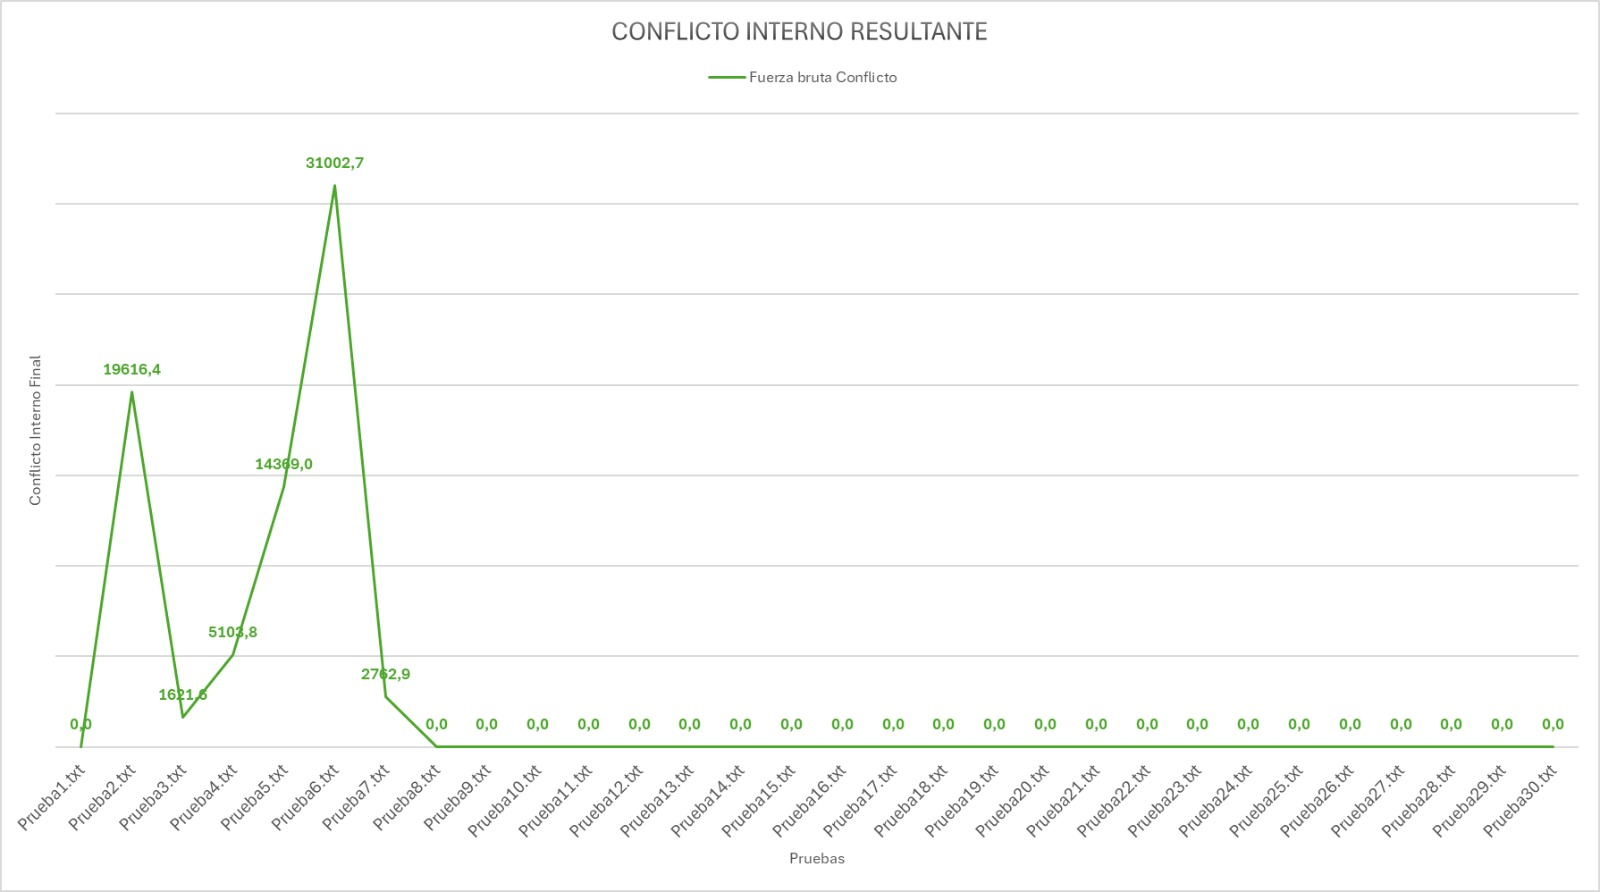
\includegraphics[width=0.8\textwidth]{resources/conflicto1.jpeg}
            \caption{Gráfica del conflicto interno generado por fuerza bruta.}
        \end{figure}
        \item \textbf{Programación dinámica:}
        \begin{itemize}
            \item Siempre encontró la solución óptima, incluso en instancias donde la fuerza bruta no completó.
            \item Solo falló en 2 pruebas, no retornando respuesta en Prueba29.txt, Prueba30.txt.
        \end{itemize}
        \begin{figure}[H]
            \centering
            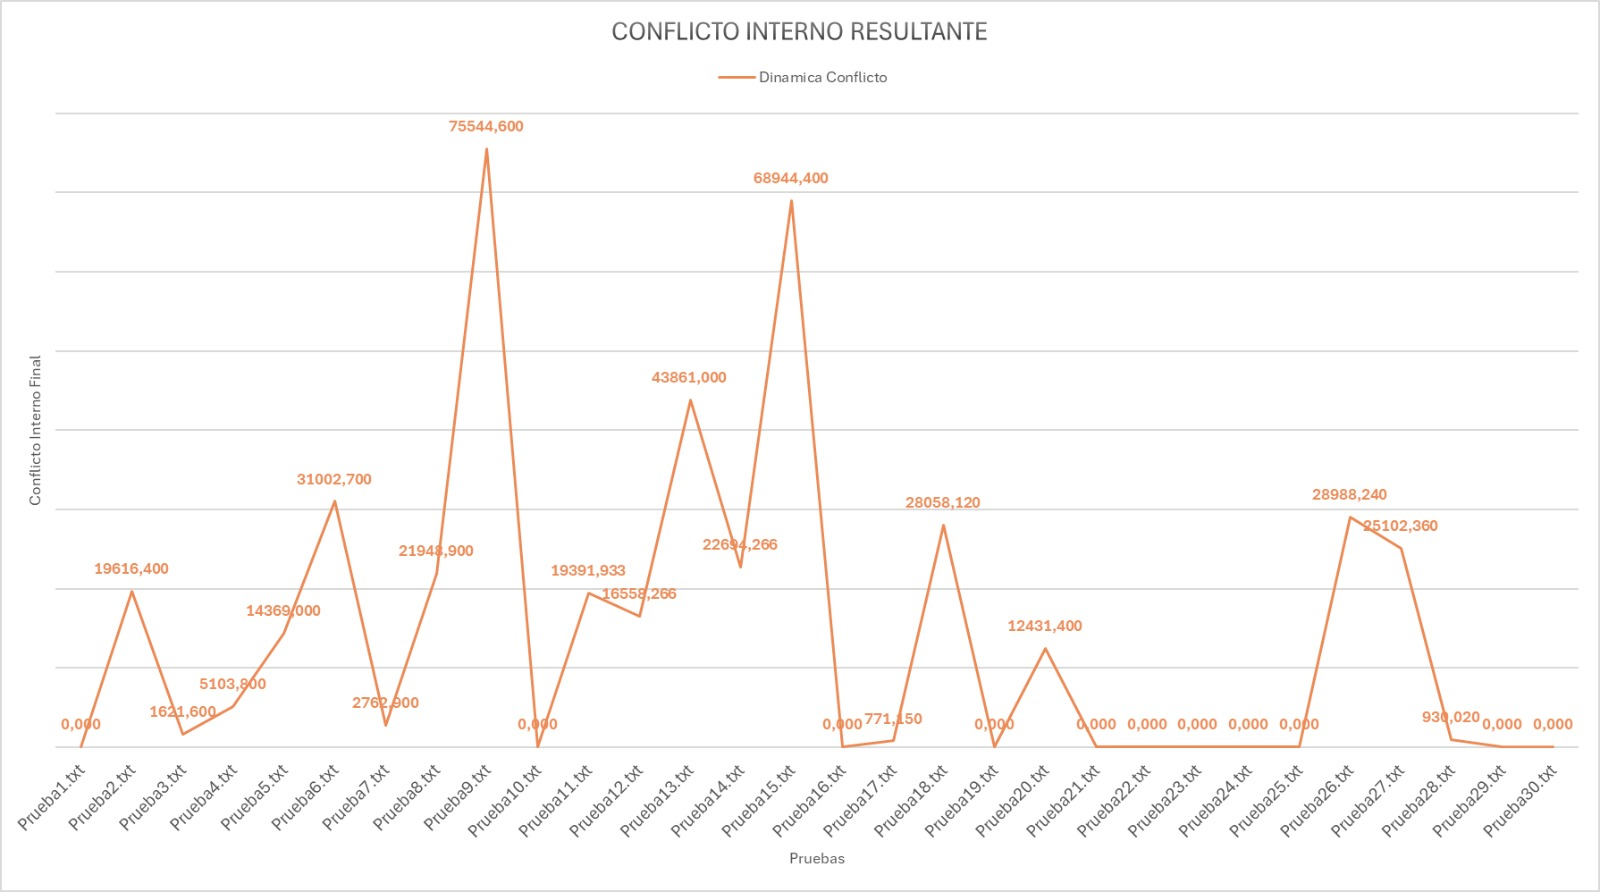
\includegraphics[width=0.8\textwidth]{resources/conflicto2.jpeg}
            \caption{Gráfica del conflicto interno generado por programación dinámica.}
        \end{figure}
        \item \textbf{Algoritmo voraz:}
        \begin{itemize}
            \item Fue el más rápido en todas las pruebas, con tiempos del orden de milisegundos.
            \item No garantiza solución óptima: en todas las pruebas arrojó una solución, pero esta no siempre coincidió con el CI mínimo real, sin embargo, en promedio difiere de la respuesta óptima que arroja la programación dinámica en un 1,62 \%.
        \end{itemize}
        \begin{figure}[H]
            \centering
            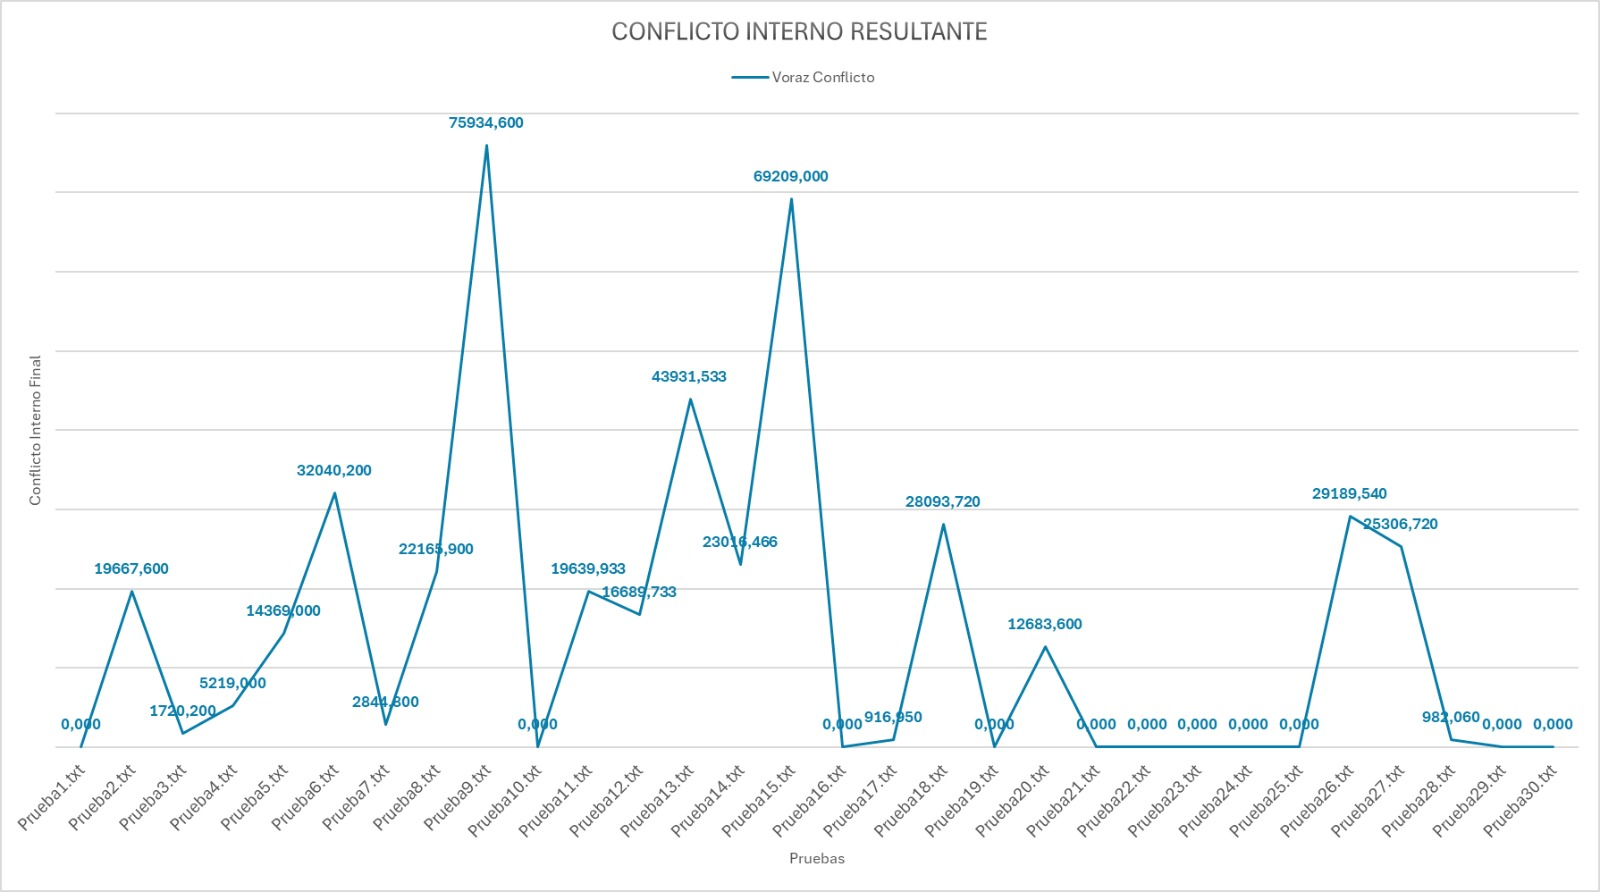
\includegraphics[width=0.8\textwidth]{resources/conflicto3.jpeg}
            \caption{Gráfica del conflicto interno generado por algoritmo voraz.}
        \end{figure}
        \begin{figure}[H]
            \centering
            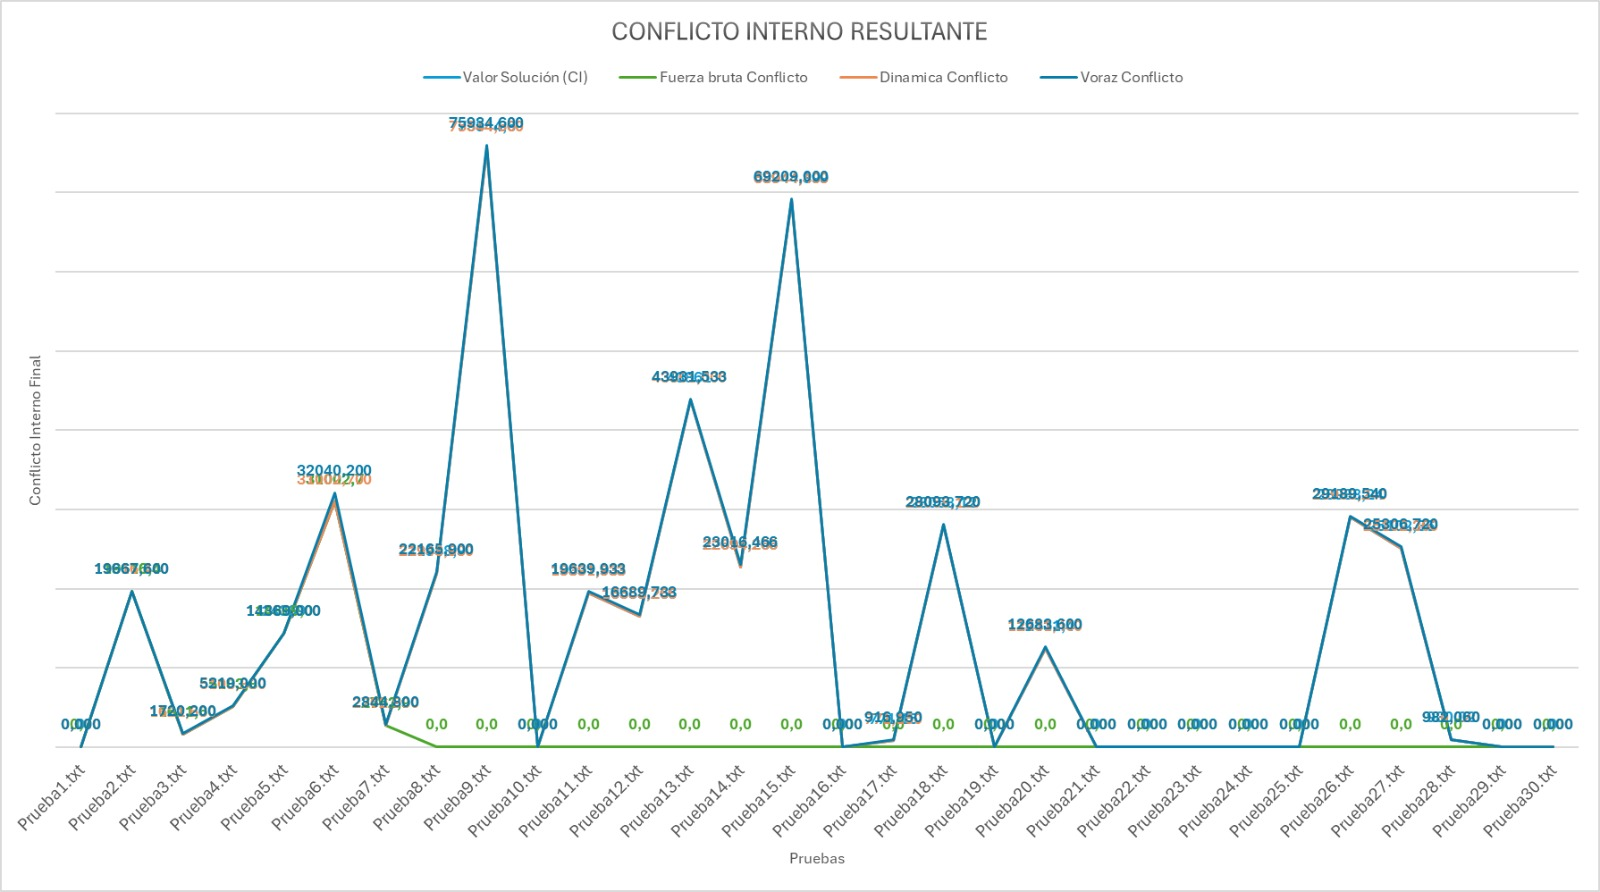
\includegraphics[width=0.8\textwidth]{resources/conflicto4.jpeg}
            \caption{Gráfica del conflicto interno comparando los tres metodos.}
        \end{figure}
    \end{itemize}

    \textbf{En resumen:}
    \begin{itemize}
        \item Fuerza bruta y dinámica aseguran la precisión máxima, pero no siempre pueden ejecutarse eficientemente.
        \item Voraz, aunque no garantiza optimalidad, ofrece soluciones rápidas y suficientemente cercanas a la óptima, incluso en escenarios con muchos agentes.
    \end{itemize}

    \subsection{Tiempos de Ejecución}

\begin{table}[H]
\centering
\begin{adjustbox}{width=\textwidth}
\begin{tabular}{|l|c|c|c|c|}
\hline
Prueba & N. Grupos de Agentes & Fuerza Bruta Tiempo seg & Dinamica Tiempo seg & Voraz Tiempo seg \\
\hline
Prueba1.txt & 5 & \cellcolor{rosado}0,0051 & \cellcolor{verde}0,0037 & \cellcolor{verde}0,0000 \\
\hline
Prueba2.txt & 5 & \cellcolor{rosado}0,0358 & \cellcolor{verde}0,0065 & \cellcolor{verde}0,0001 \\
\hline
Prueba3.txt & 5 & \cellcolor{rosado}0,0117 & \cellcolor{verde}0,0073 & \cellcolor{verde}0,0000 \\
\hline
Prueba4.txt & 5 & \cellcolor{rosado}0,0065 & \cellcolor{verde}0,0021 & \cellcolor{verde}0,0000 \\
\hline
Prueba5.txt & 5 & \cellcolor{rosado}0,0421 & \cellcolor{verde}0,0041 & \cellcolor{verde}0,0000 \\
\hline
Prueba6.txt & 10 & \cellcolor{rosado}115,9665 & \cellcolor{verde}0,0029 & \cellcolor{verde}0,0000 \\
\hline
Prueba7.txt & 10 & \cellcolor{rosado}35,1900 & \cellcolor{verde}0,0559 & \cellcolor{verde}0,0000 \\
\hline
Prueba8.txt & 10 & \cellcolor{rosado}X & \cellcolor{verde}0,5037 & \cellcolor{verde}0,0001 \\
\hline
Prueba9.txt & 10 & \cellcolor{rosado}X & \cellcolor{verde}0,4903 & \cellcolor{verde}0,0000 \\
\hline
Prueba10.txt & 10 & \cellcolor{rosado}X & \cellcolor{verde}0,9360 & \cellcolor{verde}0,0000 \\
\hline
Prueba11.txt & 15 & \cellcolor{rosado}X & \cellcolor{verde}0,9360 & \cellcolor{verde}0,0000 \\
\hline
Prueba12.txt & 15 & \cellcolor{rosado}X & \cellcolor{verde}0,0402 & \cellcolor{verde}0,0000 \\
\hline
Prueba13.txt & 15 & \cellcolor{rosado}X & \cellcolor{verde}0,5627 & \cellcolor{verde}0,0000 \\
\hline
Prueba14.txt & 15 & \cellcolor{rosado}X & \cellcolor{verde}5,1563 & \cellcolor{verde}0,0000 \\
\hline
Prueba15.txt & 15 & \cellcolor{rosado}X & \cellcolor{verde}0,7574 & \cellcolor{verde}0,0000 \\
\hline
Prueba16.txt & 20 & \cellcolor{rosado}X & \cellcolor{verde}3,3455 & \cellcolor{verde}0,0000 \\
\hline
Prueba17.txt & 20 & \cellcolor{rosado}X & \cellcolor{verde}8,9823 & \cellcolor{verde}0,0000 \\
\hline
Prueba18.txt & 25 & \cellcolor{rosado}X & \cellcolor{verde}5,4816 & \cellcolor{verde}0,0000 \\
\hline
Prueba19.txt & 25 & \cellcolor{rosado}X & \cellcolor{verde}10,1032 & \cellcolor{verde}0,0001 \\
\hline
Prueba20.txt & 25 & \cellcolor{rosado}X & \cellcolor{verde}12,4681 & \cellcolor{verde}0,0000 \\
\hline
Prueba21.txt & 50 & \cellcolor{rosado}X & \cellcolor{verde}29,3461 & \cellcolor{verde}0,0001 \\
\hline
Prueba22.txt & 50 & \cellcolor{rosado}X & \cellcolor{verde}25,0628 & \cellcolor{verde}0,0001 \\
\hline
Prueba23.txt & 50 & \cellcolor{rosado}X & \cellcolor{verde}160,8041 & \cellcolor{verde}0,0001 \\
\hline
Prueba24.txt & 50 & \cellcolor{rosado}X & \cellcolor{verde}174,4527 & \cellcolor{verde}0,0001 \\
\hline
Prueba25.txt & 50 & \cellcolor{rosado}X & \cellcolor{verde}131,9559 & \cellcolor{verde}0,0001 \\
\hline
Prueba26.txt & 50 & \cellcolor{rosado}X & \cellcolor{verde}71,8948 & \cellcolor{verde}0,0001 \\
\hline
Prueba27.txt & 100 & \cellcolor{rosado}X & \cellcolor{verde}553,2430 & \cellcolor{verde}0,0002 \\
\hline
Prueba28.txt & 100 & \cellcolor{rosado}X & \cellcolor{verde}296,0398 & \cellcolor{verde}0,0002 \\
\hline
Prueba29.txt & 100 & \cellcolor{rosado}X & \cellcolor{rosado}X & \cellcolor{verde}0,0002 \\
\hline
Prueba30.txt & 100 & \cellcolor{rosado}X & \cellcolor{rosado}X & \cellcolor{verde}0,0002 \\
\hline
\end{tabular}
\end{adjustbox}
\caption{Tiempos de ejecución para los distintos algoritmos en cada archivo de prueba}
\end{table}


    En cuanto a los tiempos, es claro en la tabla que los tiempos del algoritmo voraz son mucho menores que de los demás algoritmos. A Continuación una representación gráfica de los tiempos de los tres algoritmos:

    \begin{figure}[H]
        \centering
        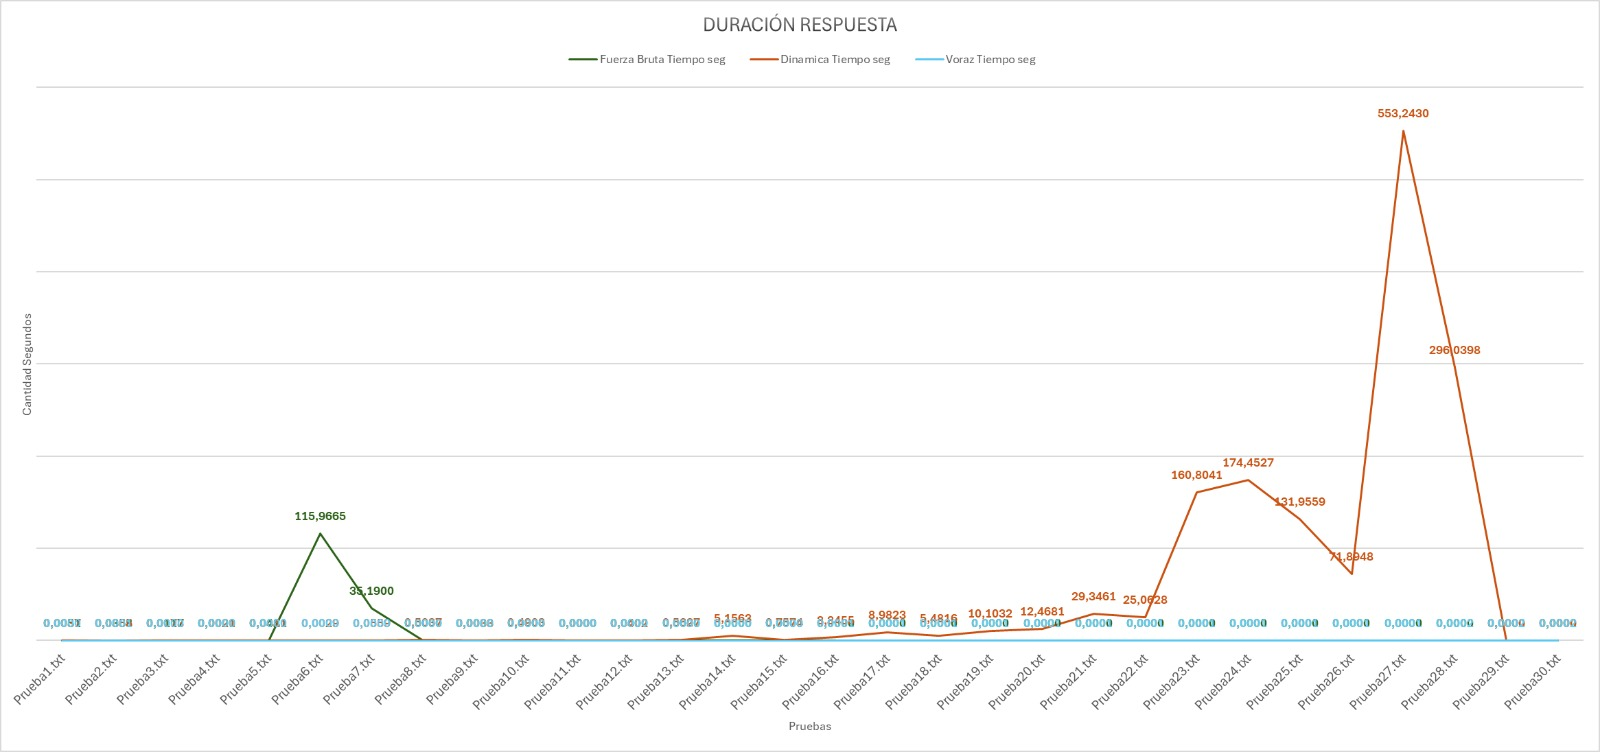
\includegraphics[width=0.8\textwidth]{resources/tiempo1.jpeg}
        \caption{Gráfica comparativa del tiempo de respuesta obtenido por cada algoritmo.}
    \end{figure}

    \begin{itemize}
        \item \textbf{Fuerza bruta:}
        \begin{itemize}
            \item Su tiempo de ejecución crece exponencialmente con el número de agentes.
            \item Aunque fue rápido para pequeños casos (5 o 10 grupos), superó los 100 segundos en algunas pruebas (Prueba6.txt) y no logró 73% de las pruebas.
        \end{itemize}
        \begin{figure}[H]
            \centering
            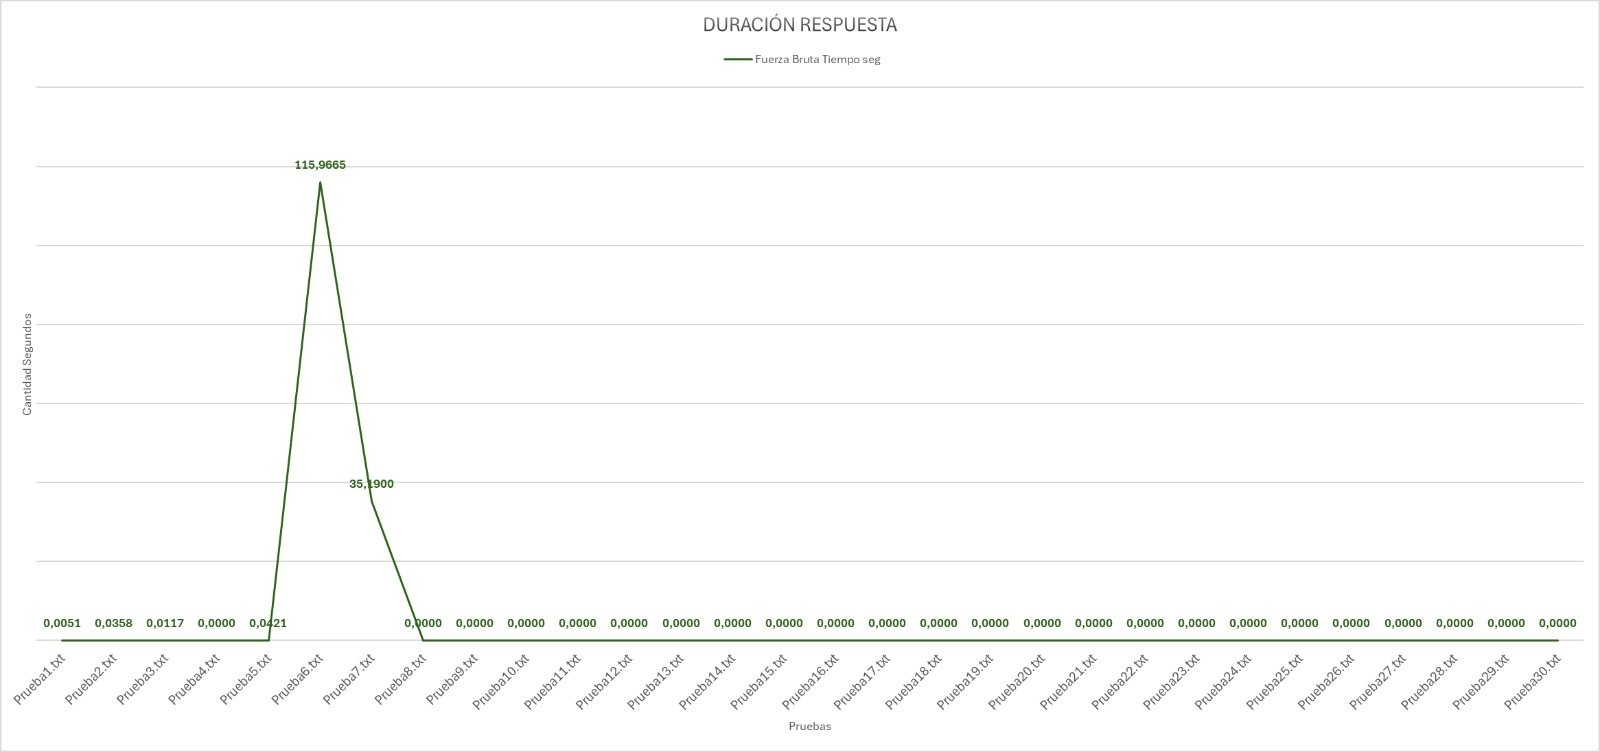
\includegraphics[width=0.8\textwidth]{resources/tiempo2.jpeg}
            \caption{Gráfica del tiempo de respuesta obtenido por fuerza bruta.}
        \end{figure}
        \item \textbf{Programación dinámica:}
        \begin{itemize}
            \item Presenta un crecimiento más moderado, pero aún significativo en problemas grandes.
            \item Tiempos mayores a 1 minuto se observaron en los archivos con más de 50 grupos.
            \item Solo falló en 2 pruebas (Prueba29.txt, Prueba30.txt), mostrando una alta escalabilidad en comparación con fuerza bruta.
        \end{itemize}
        \begin{figure}[H]
            \centering
            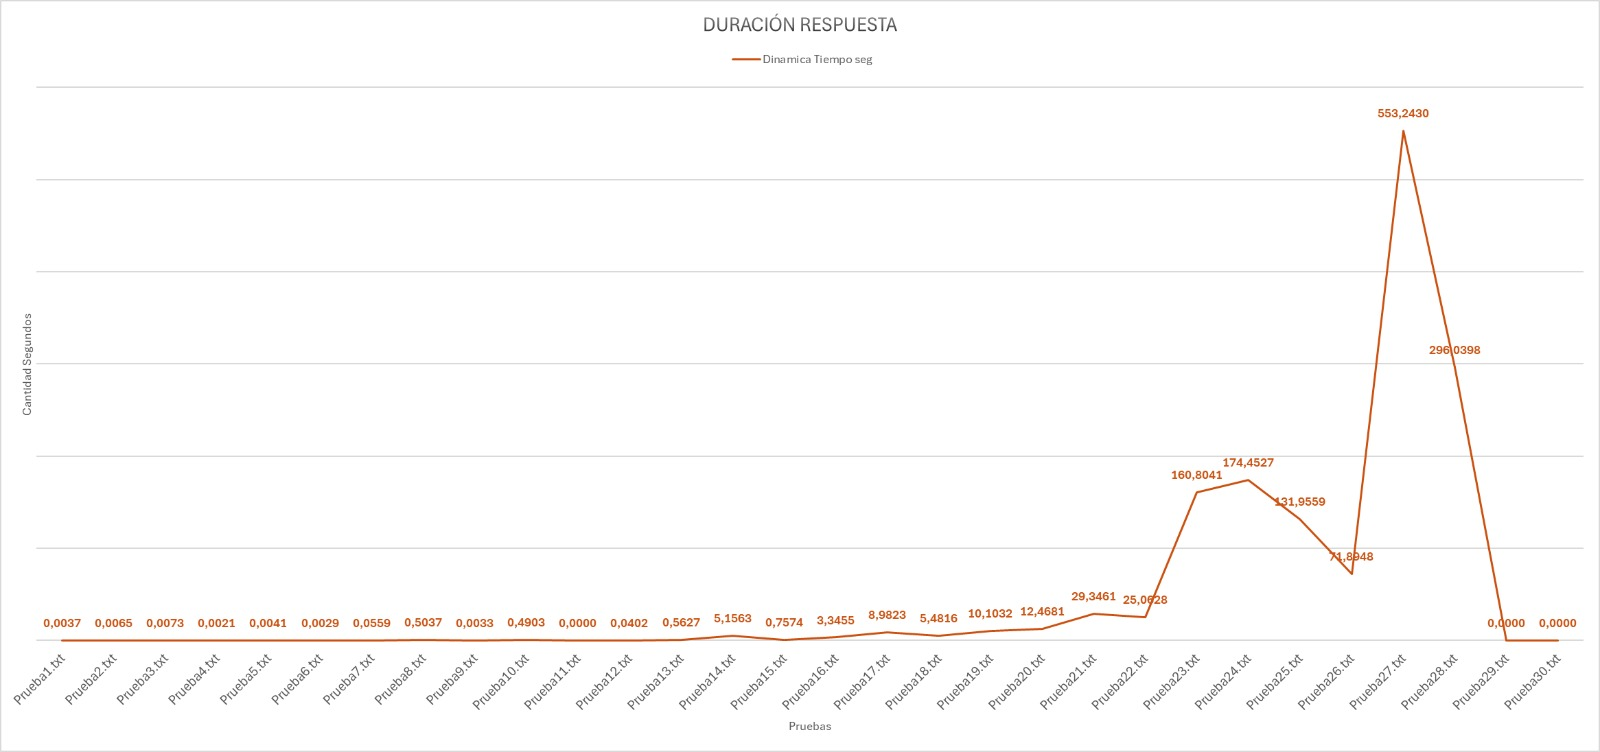
\includegraphics[width=0.8\textwidth]{resources/tiempo3.jpeg}
            \caption{Gráfica del tiempo de respuesta obtenido por programación dinámica.}
        \end{figure}
        \item \textbf{Algoritmo voraz:}
        \begin{itemize}
            \item Extremadamente eficiente en tiempo. Todos los tiempos son inferiores a 0.0003 segundos.
        \end{itemize}
        \begin{figure}[H]
            \centering
            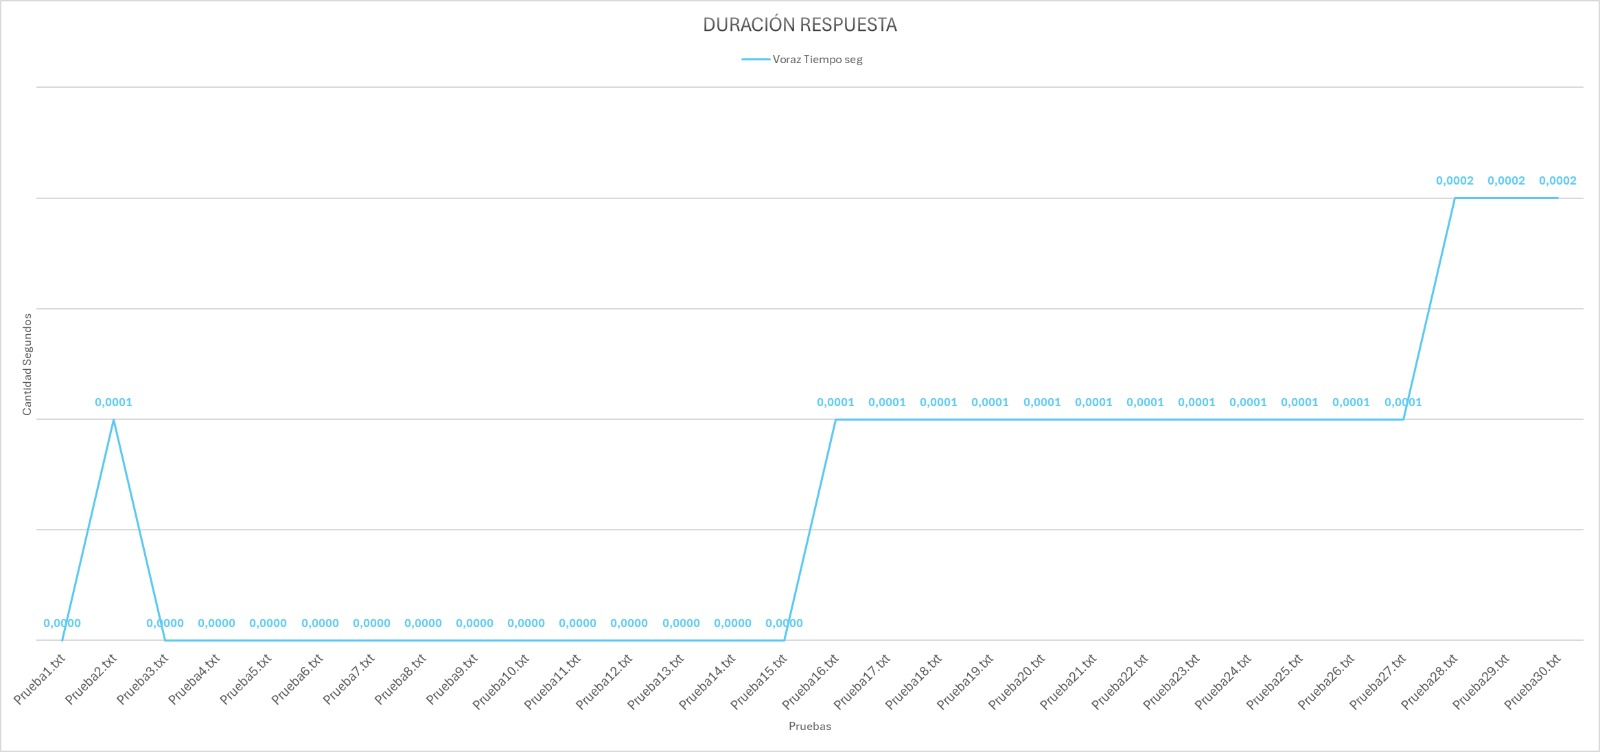
\includegraphics[width=0.8\textwidth]{resources/tiempo4.jpeg}
            \caption{Gráfica del tiempo de respuesta obtenido por algoritmo voraz.}
        \end{figure}
    \end{itemize}

    \textbf{Conclusión:}
\begin{itemize}
    \item Si se prioriza el tiempo de ejecución, el algoritmo voraz es ideal, resolviendo virtualmente al instante.
    \item Para situaciones donde la calidad de la solución es crítica, puede preferirse programación dinámica, aunque con tiempos más elevados.
    \item Fuerza bruta solo es viable para instancias pequeñas, siendo impráctico para escenarios reales por su excesivo tiempo.
\end{itemize}

La siguiente tabla presenta una comparación general entre los tres enfoques implementados: fuerza bruta, programación dinámica y algoritmo voraz. Se analizan aspectos clave como eficiencia, escalabilidad y adecuación al problema:

\begin{table}[H]
    \centering
    \renewcommand{\arraystretch}{1.5}
    \begin{tabular}{C{4cm} C{3cm} C{3.5cm} C{3.5cm}}
        \toprule
        \textbf{Criterio}                              & \textbf{Fuerza Bruta}                   & \textbf{Programación Dinámica} & \textbf{Algoritmo Voraz}              \\
        \midrule
        Complejidad Temporal                           & \( O(n(k+1)^n) \)                       & \(O(n \cdot R_{\text{real}} \cdot k_{\text{real}})\)                 & \( O(n \log n) \)                     \\
        Complejidad Espacial                           & \( O((k+1)^n) \)                        & \( O(n^2 \times R_{max} \times k)\)                 & \( O(n) \)                            \\
        ¿Siempre da la solución óptima?                & Sí                                      & Sí                             & No                                    \\
        ¿Es capaz de manejar gran cantidad de agentes? & No                                      & Moderada                 & Alta                                  \\
        Aplicación recomendada                         & Problemas pequeños                      & Problemas moderados                      & Problemas grandes                     \\
        Eficiencia en Tiempo                           & Muy baja (crece exponencialmente)       & Moderada (tiempo polinomial)                      & Alta (tiempo lineal o logarítmico)    \\
        Eficiencia en Espacio                          & Muy baja, requiere mucho almacenamiento & Moderada, requiere una cantidad de almacenamiento moderada                      & Alta, requiere poco espacio adicional \\
        \bottomrule
    \end{tabular}
    \caption{Comparación general entre algoritmos.}
\end{table}

    \textbf{Análisis general:}
    \begin{itemize}
        \item \textbf{Fuerza Bruta} es útil como referencia o verificación para instancias pequeñas. Su exactitud es total, pero su alto costo computacional limita su uso práctico a casos muy reducidos.
        \item \textbf{Programación Dinámica} logra mantener la precisión y mejorar la eficiencia respecto a la fuerza bruta. Aun así, su uso intensivo de memoria y tiempo en casos grandes representa una limitación.
        \item \textbf{Algoritmo Voraz}, aunque no garantiza la solución óptima, ofrece resultados de buena calidad en tiempos extremadamente bajos, por lo que es ideal para escenarios donde se necesita una respuesta rápida y lo más cercana a la óptima.
    \end{itemize}

    \subsection{Ventajas y Desventajas}

    El análisis de los tres algoritmos propuestos para resolver el problema de moderación del conflicto interno en redes sociales permite establecer comparaciones fundamentales en cuanto a precisión, eficiencia y aplicabilidad práctica. A continuación, se sintetizan las ventajas y desventajas más relevantes de cada enfoque:

    \subsubsection{Fuerza Bruta}

    \begin{itemize}
        \item \textbf{Ventajas:}
        \begin{itemize}
            \item Garantiza encontrar la solución óptima, al evaluar todas las posibles combinaciones.
            \item Es útil como referencia o punto de comparación para validar otros algoritmos aproximados.
            \item Implementación directa y sencilla desde el punto de vista conceptual.
        \end{itemize}
        \item \textbf{Desventajas:}
        \begin{itemize}
            \item Su complejidad temporal es exponencial, lo que lo vuelve inviable para instancias grandes.
            \item Requiere un tiempo de ejecución considerable incluso para tamaños de entrada moderados.
            \item No escala con eficiencia a redes sociales reales con cientos o miles de agentes.
        \end{itemize}
    \end{itemize}

    \subsubsection{Programación Dinámica}

    \begin{itemize}
        \item \textbf{Ventajas:}
        \begin{itemize}
            \item  Debido a que se divide el problema en subproblemas y se resuelve cada uno, se garantiza encontrar la solución óptima, en las pruebas realizadas, la solución siempre es la óptima como se puede ver.
            \item  La complejidad espacial es reducida significativamente a diferencia de fuerza bruta.
            \item Se evita hacer cálculos repetidos ya que utiliza los que ya ha hecho en otros subproblemas, haciendolá más adecuada para redes medianas y grandes donde se requiere precisión y rendimiento.
        \end{itemize}
        \item \textbf{Desventajas:}
        \begin{itemize}
            \item  Aunque su complejidad temporal mejora, se ve afectado el espacio en memoria, la complejidad espacial, con el fin de almacenar las soluciones parciales
        \end{itemize}
    \end{itemize}

    \subsubsection{Voraz}

    \begin{itemize}
        \item \textbf{Ventajas:}
        \begin{itemize}
            \item  Su ejecución es rápida y consume pocos recursos, ideal para entornos donde el tiempo de respuesta es crítico.
            \item  La implementación es sencilla y generalmente más comprensible.
            \item Escala bien para redes sociales grandes.
        \end{itemize}
        \item \textbf{Desventajas:}
        \begin{itemize}
            \item  No garantiza obtener la solución óptima, ya que toma decisiones locales sin evaluar el impacto global.
        \end{itemize}
    \end{itemize}

     \vspace{1em}
    \noindent
    \begin{tcolorbox}[colback=red!5!white, colframe=red!50!black, title=Comparación Global]
        El algoritmo de fuerza bruta actúa como una línea base teórica inigualable en precisión, pero ineficiente. La programación dinámica logra un balance adecuado entre eficiencia y exactitud, mientras que el enfoque voraz se justifica principalmente cuando se requiere velocidad y se puede tolerar una aproximación. La elección del algoritmo adecuado dependerá del tamaño del problema, los recursos disponibles y el nivel de precisión requerido por la aplicación práctica.
    \end{tcolorbox}

    

%%%%%%% COMPARACIÓN ALGORITMOS %%%%%%% FIN

    \newpage

%%%%%%% CASOS DE PRUEBA %%%%%%% INICIO


    \section{Casos de Prueba}

    Se realizan casos de prueba para los diferentes tipos de algoritmos (fuerza bruta, programación dinámica y voraz) con el objetivo de evaluar su eficiencia, exactitud y comportamiento en diversas condiciones. Esto permite comparar qué algoritmo es más eficiente en determinados casos, poniendo a prueba su desempeño en situaciones donde el uso de memoria y capacidad de procesamiento son claves para su correcto funcionamiento. Se han llevado a cabo los siguientes casos de pruebas:

\subsection{Caso de Prueba 1}
\begin{figure}[H]
    \centering
    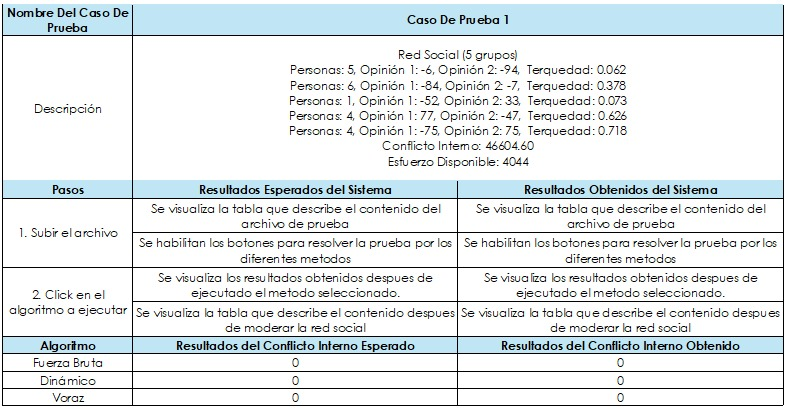
\includegraphics[width=\linewidth]{resources/cp1.jpeg}
    \caption{Caso de Prueba 1}
    \label{fig:cp1}
\end{figure}

\subsection{Caso de Prueba 2}
\begin{figure}[H]
    \centering
    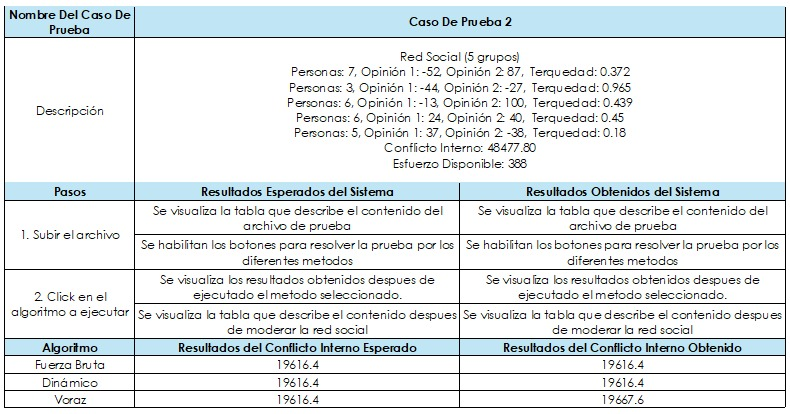
\includegraphics[width=\linewidth]{resources/cp2.jpeg}
    \caption{Caso de Prueba 2}
    \label{fig:cp2}
\end{figure}

\subsection{Caso de Prueba 3}
\begin{figure}[H]
    \centering
    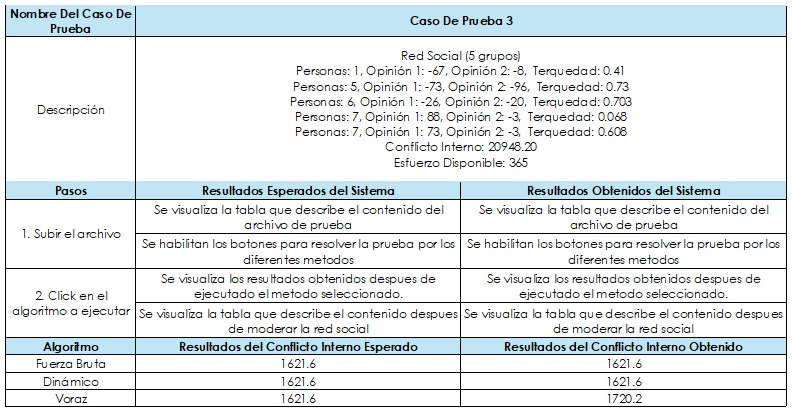
\includegraphics[width=\linewidth]{resources/cp3.jpeg}
    \caption{Caso de Prueba 3}
    \label{fig:cp3}
\end{figure}

\subsection{Caso de Prueba 4}
\begin{figure}[H]
    \centering
    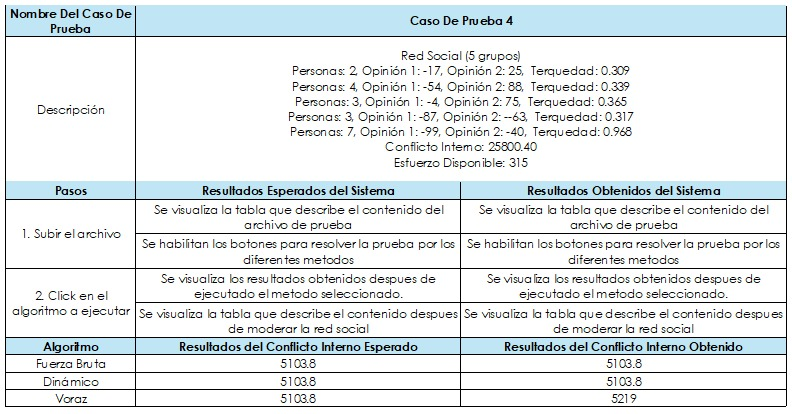
\includegraphics[width=\linewidth]{resources/cp4.jpeg}
    \caption{Caso de Prueba 4}
    \label{fig:cp4}
\end{figure}

\subsection{Caso de Prueba 5}
\begin{figure}[H]
    \centering
    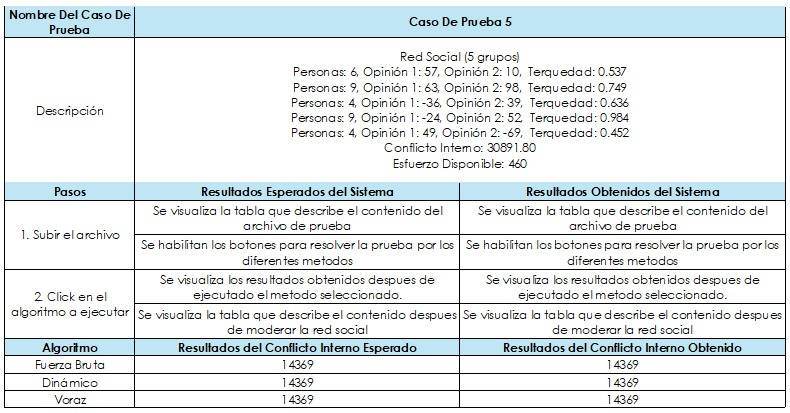
\includegraphics[width=\linewidth]{resources/cp5.jpeg}
    \caption{Caso de Prueba 5}
    \label{fig:cp5}
\end{figure}


%%%%%%% CASOS DE PRUEBA %%%%%%% FIN

\newpage

\section{Conclusiones}

\begin{itemize}
    \item \textbf{El algoritmo de fuerza bruta}: garantiza encontrar la solución óptima al problema, ya que explora exhaustivamente todas las combinaciones posibles de esfuerzo entre los grupos. Sin embargo, su principal desventaja es la complejidad exponencial, lo que lo hace inviable para redes con más de unos pocos grupos. En la práctica, su uso queda restringido a casos muy pequeños, donde se puede usar como referencia o para validar otros métodos.
    
    \item \textbf{El algoritmo de programación dinámica}: representa una mejora significativa en cuanto a eficiencia respecto al enfoque de fuerza bruta. Se basa en subproblemas más pequeños y permite reutilizar resultados intermedios, logrando una solución óptima dentro del presupuesto de esfuerzo. A pesar de que su complejidad temporal y espacial sigue siendo considerable, su rendimiento es aceptable en redes medianas, incluso con restricciones de tiempo o memoria. Permite alcanzar un equilibrio entre exactitud, rendimiento y escalabilidad.
    
    \item \textbf{El algoritmo voraz}: es el más rápido de los tres, ya que se basa en una heurística que prioriza grupos con alta discrepancia de opiniones y baja rigidez. Aunque no garantiza una solución óptima, ofrece resultados suficientemente buenos en tiempos muy bajos. Su bajo costo computacional lo hace ideal para redes grandes o situaciones donde se requiere una respuesta rápida. Sin embargo, su eficacia depende fuertemente de la calidad de la heurística utilizada, y puede no funcionar bien en ciertos casos.
    
    \item \textbf{En conclusión}: el análisis comparativo evidencia que cada enfoque tiene su nicho de aplicabilidad. La fuerza bruta es útil solo para instancias pequeñas y como referencia. La programación dinámica es preferible cuando se necesita precisión y aún se dispone de recursos moderados. El enfoque voraz es el más adecuado cuando se busca eficiencia y rapidez en contextos de gran escala. La elección del algoritmo debe estar guiada por el tamaño de la red, el presupuesto disponible y el nivel de precisión requerido.
\end{itemize}


\newpage

\section{Ejecución del proyecto}

La ejecución de este proyecto se apoya en contenedores Docker para garantizar un entorno aislado y reproducible. A continuación, se detallan los pasos necesarios para clonar, construir y lanzar la aplicación, tanto en sistemas Windows como Linux/macOS.

\subsection*{1. Clonar el repositorio}

Abra una terminal o consola de comandos y ejecute:

\begin{verbatim}
git clone https://github.com/Ajred96/ProyectoIADAII.git
cd ProyectoIADAII
\end{verbatim}

\subsection*{2. Instalar Docker y Docker Compose}

Antes de continuar, asegúrese de tener instalado Docker en su sistema.

\begin{itemize}
    \item \textbf{Windows:} Instalar desde \url{https://www.docker.com/products/docker-desktop}
    \item \textbf{Linux/macOS:} Seguir instrucciones en \url{https://docs.docker.com/engine/install/}
\end{itemize}

Una vez instalado, puede verificar la instalación ejecutando:

\begin{verbatim}
docker --version
docker compose version
\end{verbatim}

\subsection*{3. Construir y ejecutar el proyecto}

Desde la raíz del proyecto, ejecute el siguiente comando para construir e iniciar los contenedores:

\begin{verbatim}
docker compose up --build
\end{verbatim}

Este comando descargará las imágenes necesarias y levantará automáticamente los servicios de la aplicación.

\subsection*{4. Acceder a la aplicación}

Una vez que todos los servicios estén corriendo, la interfaz estará disponible en su navegador en:

\begin{verbatim}
http://localhost:4200
\end{verbatim}

\noindent
La aplicación quedará lista para ser utilizada sin necesidad de configuración adicional.


\newpage
\nocite{*}
\printbibliography

\end{document}